% ------------------------------------------------------------------------------
% Proposed Methodology
% ------------------------------------------------------------------------------

\chapter{Proposed Methodology}\label{chap:proposed-methodology}

	This thesis aims to enhance the current state-of-the-art algorithms for microwave imaging by proposing novel approaches based on surrogate models. Additionally, a comprehensive framework for the development and testing of algorithms specific to this problem is presented. In Section \ref{chap:proposed-methodology:criticism}, a critical review of the literature is presented, highlighting the gaps and areas for improvement in the current state of the art. Building on this analysis, Section \ref{chap:proposed-methodology:proposal} proposes a novel approach to address some of the limitations, specifically, the use of surrogate models and the framework for development and comparison of algorithms designed for EISPs. Section \ref{chap:proposed-methodology:surrogate} provides a detailed discussion of surrogate-model assisted algorithms for microwave imaging, including a description of the transformation of the inversion problem into a bidimensional optimization one, the Kriging model, and the proposed algorithms. Section \ref{chap:proposed-methodology:library} outlines a framework for developing and testing algorithms for microwave imaging, including the proposed metrics to assess their performance. Finally, Section \ref{chap:proposed-methodology:conclusion} presents the concluding remarks.

	\section{Literature Criticism and Opportunities}\label{chap:proposed-methodology:criticism}
	
		In the early stages of developing algorithms for microwave imaging, several challenges were encountered \citep{kirsch2011introduction,pastorino2000microwave,bertero2020introduction}. In the early context, the available data was significantly limited and noisy, which represented a serious challenge for a problem with non-unique solution. When more data was available, the limited computing power was other challenge. The understanding of the physics involved in microwave imaging also evolved throughout the years, which was also important for the development of the subject.
	
		Currently, two significant challenges are faced by researchers in the literature: real-time imaging and the retrievement of strong scatterers. Real-time imaging requires fast and efficient algorithms that can produce accurate images in real-time or nearly, which is essential for many applications such as medical imaging \citep{li2021machine} and security screening \citep{asok2022concealed}. To address this challenge, researchers have turned to deep-learning techniques that can efficiently process large amounts of data and provide accurate results in real-time \citep{salucci2022artificial}.
		
		The other challenge is the imaging of strong scatterers, which refers to objects with high contrast levels or large dimensions when comparing to the wavelength. Such objects result in high nonlinearity and can create significant artifacts in the resulting image, making it difficult to accurately reconstruct the underlying structure. This is particularly challenging when imaging complex structures, such as biological tissues or composite materials \citep{lazebnik2007large}. This type of scenario has been addressed in three main ways:
		\begin{enumerate}
			\item The first approach is to reduce the degree of non-linearity by changing the integrals solved by the algorithms (Section \ref{chap:problemstatement:eisp});
			\item The second approach is based on domain decomposition \citep{zhang2022iterative}. This approach divides the scatterer region into dominant and subordinate subdomains based on the information of the induced current. The dominant subdomain is then reconstructed iteratively, narrowing the inversion domain and reducing the nonlinearity of the problem.
			\item The third approach is the use of surrogate models \citep{koziel2008engineering}. \cite{salucci2022learned} proposed a surrogate model to predict the data equation error considering curve-based representations of scatterers. By using this approach, the computational cost of stochastic algorithms that do not solve the contrast and the total field simultaneously can be significantly reduced. This is because such algorithms rely on forward problem simulations to estimate the error. The authors demonstrated the effectiveness of their approach in high-contrast scenarios, showing promising results.
		\end{enumerate}
		
		Some ideas in the field have yet to receive the attention they deserve, and one of them is the use of qualitative methods to define initial solutions for quantitative algorithms. Even though this approach has been explored in some papers \citep{zhang2020learning,han2022hybrid,bevacqua2015algebraic}, it has yet to be fully utilized to improve the performance of stochastic algorithms for the problem. The use of qualitative methods can help to improve the robustness of images reconstructed by these algorithms to noise and high contrasts, as well as guide the convergence of population-based algorithms towards more promising regions of the search space.
		
		%Outro aspecto que chama a atenção na literatura é o design dos experimentos e a avaliação da qualidade dos algoritmos. É necessário destacar que um aspecto extremamente relevante para a experimentação é a utilização de modelos de espalhadores mais realísticos ou dados obtidos de medições reais. Isto tem ficado popular na literatura através laboratórios que disponibilização os dados. Dois exemplos muito comuns são o \textit{UWCEM Numerical Breast Phantom Repository} \citep{burfeindt2012mri} e as medições realizadas pelo \textit{Institut Fresnel} \citep{geffrin2005free}. 
		Another aspect that draws attention in the literature is experiment design and quality evaluation of algorithms. A highly relevant aspect of experimentation is using more realistic scatterer models or data obtained from real measurements. This has become popular in the literature through laboratories that make the data available. Two widespread examples are the \textit{UWCEM Numerical Breast Phantom Repository} \citep{burfeindt2012mri}  and the measurements made by the \textit{Institut Fresnel} \citep{geffrin2005free}.
		
		In addition, \cite{kurrant2021evaluating} have recently proposed a methodology to evaluate the performance of the algorithms applied to breast cancer detection. Given a reference image and the recovered one, the authors proposed to segment the tissues in the images by an unsupervised machine learning approach. After decomposing the images and mapping the tissues, five metrics were proposed to evaluate shape fidelity, malignant tissue reconstruction in tumor regions, among others. Therefore, the novelty is a technique to measure the quality of breast reconstruction with suitable tools. Their methodology is also available as a MATLAB toolbox \citep{kurrant2021mwsegeval}.
		
		%No entanto, os autores das publicações tradicionalmente escolhem instâncias com características particulares com o objetivo de demonstrar a capacidade de reconstrução do método proposto na correspondente situação. A partir disso, a performance é medida através de algum indicador de qualidade e o resultado é comparado a outros algoritmos e formulações \citep{zhong2020multiresolution,zhang2020wavelet,zhou2021improved}. Embora essa abordagem seja interessante para ilustrar a capacidade do algoritmo, ela tem pouco rigor metodológico para oferecer respostas robustas à perguntas como: (i) qual impacto da escolha da instância no valor do quantificador da performance? (ii) Como o indicador varia se a geometria do objeto mudar? (iii) Como a diferença na performance observada entre os dois métodos varia se as geometrias variarem? (iv) Qual a performance média ou pior caso do método para uma dada configuração? (v) Etc.
		However, in many publications addressing general applications, traditional instances have been chosen with particular characteristics to demonstrate the reconstruction ability of the proposed method in the corresponding situation. Performance is measured through some quality indicator, and the result is compared to other algorithms and formulations \citep{zhong2020multiresolution,zhang2020wavelet,zhou2021improved}. Although this approach is interesting to illustrate the algorithm's suitableness, it has little methodological rigor to offer robust answers to questions such as: (i) what is the impact of the choice of the instance on the performance quantifier's value? (ii) How does the indicator vary if the object's geometry changes? (iii) How does the difference in performance observed between the two methods vary if the geometries vary? (iv) What is the average or worst-case performance of the method for a given configuration? Among others.
		
		%Mesmo que essas perguntas possam fugir do escopo de propostas baseadas em um estudos de caso (e.g., experimentos reais), conclusões gerais sobre a capacidade e performance podem ser muito fracas sem uma metodologia experimental adequada que leve em consideração diferentes fatores de efeito na configuração do problema. Embora o fator de nível de ruído costume ser o mais explorado nesse sentido \citep{chew1990reconstruction,chen2010subspace,shah2018fast,batista2021quadratic}, uma experimentação com instâncias aleatórias para uma medição mais robusta da performance não foi levada em consideração nem quando a publicação tinha como objetivo principal a comparação entre algoritmos \citep{moghaddam1991comparison,gilmore2009comparison,pan2010comparison}. Este tipo de prática é essencial para eliminar o viés do observador em análises de algoritmos \citep{montgomery2010applied}. Um outro exemplo sobre isso é a existência de vários trabalhos na literatura que propõem metodologias estocásticas e nem ao menos informam quantas vezes o algoritmo foi repetido quando exibem o resultado para uma dada instância. Não há informação se o resultado mostrado representa o pior, médio ou melhor caso, como se fosse o resultado único de um tipo de metodologia que não tem garantia nenhuma de retornar a mesma solução em toda execução \citep{massa2005parallel,ashtari2010using,salucci2017multifrequency}.
		Even though these questions may fall outside the scope of proposals based on case studies (e.g., physical experiments), general conclusions about suitability and performance can be very weak without an adequate experimental methodology that considers different effect factors in the configuration of the problem. Although the noise level factor is usually the most explored in this sense \citep{chew1990reconstruction,chen2010subspace,shah2018fast,batista2021quadratic}, experiments with random instances for a more robust measurement performance are not usually performed. Even when the publication had the main objective of comparing algorithms \citep{moghaddam1991comparison,gilmore2009comparison,pan2010comparison}. This practice is essential to eliminate the observer's bias in algorithms analysis \citep{montgomery2010applied}. Other examples are several works in the literature that propose stochastic methodologies and do not even inform how many times the algorithm was repeated when showing the result for a given instance. There is no information if the result shown represents the worst, average, or best case. This is problematic since these methodologies have no guarantee of returning the same solution in every execution \citep{massa2005parallel,ashtari2010using,salucci2017multifrequency}.
		
		%Por isso, uma oportunidade na literatura é introduzir comparações mais robustas entre algoritmos. Uma referência sobre boas práticas de comparação de algoritmos de otimização é o artigo escrito por \cite{beiranvand2017best}. Entre muitos apontamentos relevantes feitos pelos os autores, destacamos os seguintes:
		Therefore, another opportunity in the literature is to introduce more robust comparisons between algorithms, i.e., benchmarking. A reference on best practices for comparing optimization algorithms is the article written by \cite{beiranvand2017best}. Among the many relevant notes made by the authors, we highlight the following:
		
		\begin{itemize}
			%\item Um conjunto de teste com poucos problemas deve ser referido como um estudo de caso ou prova de conceito, mas não benchmarking.
			%\item Um conjunto de teste deve evitar as seguintes deficiências: (i) poucos problemas; (ii) pouca ou excessiva variação na complexidade das instâncias inviabilizando a extração de informações úteis; (iii) problemas sem soluções conhecidas (o qual pode ser inevitável em situações reais); (iv) viés no ponto de partida dos algoritmos; (v) estruturas escondidas (e.g., arredondamento de números). 
			%\item Todos algoritmos devem receber a mesma quantidade de informação de entrada e garantir que não há um pressuposto que é respeitado somente por um dos algoritmos.
			\item A test suite with few problems should be referred to as a case study or proof of concept, but not benchmarking.
			\item A test suite should avoid the following deficiencies: (i) few problems; (ii) slight or excessive variation in the complexity of the instances, making it impossible to extract helpful information; (iii) problems with no known solutions (which can be inevitable in real situations); (iv) bias at the starting point of the algorithms; (v) hidden structures.
			\item All algorithms must receive the same amount of input information and ensure that there is an assumption that is only respected by one of the algorithms in order to verify the influence of that assumption.
		\end{itemize}
		
		%Esses tópicos não representam necessariamente falhas nas experimentações descritas na literatura. No entanto, esses conceitos já estabelecidos na literatura sobre otimização podem trazer amadurecimento na de algoritmos para EISP.
		These topics do not necessarily represent failures in the experiments described in the literature. However, these concepts already established in the optimization literature can bring maturity to the algorithms for EISP.
		
		%Por fim, destacamos também as métricas utilizadas para avaliar a qualidade das reconstruções. Na vasta maioria dos trabalhos, a qualidade das imagens reconstruídas da função contraste é quantificada por uma das seguintes formas \citep{wang1989iterative,chew1990reconstruction,shah20193d,oliveri2019compressive,oliveri2011multiresolution,salucci2017multifrequency,zhang2020learning}:
		Finally, we also highlight the metrics used to assess the quality of the reconstructions. In the vast majority of works, the quality of the reconstructed images of the contrast function is quantified in one of the following ways \citep{wang1989iterative,chew1990reconstruction,shah20193d,oliveri2019compressive,oliveri2011multiresolution,salucci2017multifrequency,zhang2020learning}:
		\begin{align}
			\zeta_{\epsilon} &= \sqrt{\frac{1}{N_IN_J}\sum\limits_{i=1}^{I}\sum\limits_{j=1}^J\left|\frac{\epsilon^*_{r,ij}-\epsilon_{r,ij}}{\epsilon^*_{r,ij}}\right|^2} \label{eq:4:error0:epsilon} \\
			\zeta_{\chi} &= \sqrt{\frac{1}{N_IN_J}\sum\limits_{i=1}^{I}\sum\limits_{j=1}^J\left|\frac{\chi^*_{ij}-\chi_{ij}}{\chi^*_{ij}+1}\right|^2} \label{eq:4:error0:chi}
		\end{align}
		
		%\noindent onde $\epsilon^*_{r,ij}$ e $\chi^*_{ij}$ são os valores verdadeiros de permissividade relativa e contraste, respectivamente. Ou seja, de um modo geral, \eqref{eq:4:error0:epsilon} e \eqref{eq:4:error0:chi} são fórmulas baseadas na raiz da média do erro percentual. Pequenas variações nelas também podem ser adotadas, como a substituição de $N_IN_J$ pela área da imagem ou pela remoção da raiz e do quadrado do erro.
		\noindent where $\epsilon^*_{r,ij}$ and $\chi^*_{ij}$ are the actual values of relative permittivity and contrast, respectively. In general, \eqref{eq:4:error0:epsilon} and \eqref{eq:4:error0:chi} are formulas based on the root of the average percentage error. Slight variations can also be adopted, such as replacing $N_IN_J$ with the image area or removing the root and square of the error.
		
		%De um modo geral, quando se trata de identificar objetos na imagem, uma boa reconstrução é caracterizada pela identificação correta da posição, da forma e do contraste do espalhador. \eqref{eq:4:error0:epsilon} e \eqref{eq:4:error0:chi} são métricas que abordam essas três características ao mesmo. Uma reconstrução igual à verdadeira vai minimizar esses indicadores. No entanto, existem situações nas quais esses indicadores não são tão eficientes. Quando a área de um espalhador é muito menor que a da figura, o erro vai ser bem pequeno mesmo que haja muitos desvios na estimativa do contraste na área do espalhador (e.g., $\chi=0$). Isto pode também disfarçar erros significativos na posição e forma dos espalhadores reconstruídos. Vale à pena notar que os resíduos das equações não são tomados necessariamente como medidores de qualidade tendo em vista que, por causa da má-posição do problema, podem haver soluções com baixo resíduos e imagens diferentes das esperadas.
		In general, when it comes to identifying objects in the image, a good reconstruction is characterized by the correct identification of the scatterer's position, shape, and contrast. \eqref{eq:4:error0:epsilon} and \eqref{eq:4:error0:chi} are metrics that address these three characteristics at the same time. A reconstruction equal to the actual one will minimize these indicators. However, there are situations in which these indicators are not as efficient. When the area of a scatterer is much smaller than the figure, the error will be minimal. This might happen even if there are many deviations in the estimate of the contrast in the scatterer area (e.g., $\chi=0$). This can also disguise significant errors in the position and shape of the rebuilt scatterers. It is worth noting that the residuals of the equations are not necessarily taken as quality meters, given that, due to ill-posedness, there may be solutions with low residues and images that are different from those expected.
		
		%Conforme sugerido por \cite{beiranvand2017best}, outros indicadores também podem avaliar aspectos interessantes do desempenho dos algoritmos: (i) taxa de sucesso, i.e., quantidade de vezes que um algoritmo atinge uma determinada tolerância em um determinado tempo-limite; (ii) percentual de soluções encontradas em uma dada situação; (iii) perfil de precisão, i.e., porcentagem de problemas que um algoritmo consegue resolver para um dado percentual de precisão; (iii) perfil de performance, i.e., probabilidade que um algoritmo resolva um problema dado um limite de tempo; entre outros. Estes indicadores poderiam fornecer informações enriqueceriam muito a comparação dos algoritmos.
		As suggested by \cite{beiranvand2017best}, other indicators can also evaluate interesting aspects of algorithms performance: (i) success rate, i.e., the number of times that an algorithm reaches a certain tolerance in a specific time limit; (ii) percentage of a class of solutions found in a given situation; (iii) accuracy profile, i.e., percentage of problems that an algorithm can solve for a given percentage of accuracy; (iii) performance profile, i.e., the probability that an algorithm will solve a problem given a time limit; among others. These indicators could provide information that would greatly enrich the comparison of the algorithms.
	
	\section{Proposal}\label{chap:proposed-methodology:proposal}
	
		%Levando em consideração a discussão na seção anterior sobre o estado-da-arte e das oportunidades das lacunas presentes na literatura, esta pesquisa tem duas propostas de contribuição: (i) o projeto de algoritmos assistidos por modelos substitutos que se baseiam nas imagens geradas por métodos qualitivativos e (ii) o projeto de um software especializado para o desenvolvimento e testagem de algoritmos para o problema, com suporte a testagem randomizada e medição de performance média através de um conjunto de indicadores. Portanto, o objetivo é explorar uma nova possibilidade de aplicação de modelos substitutos que aproveite das vantagens do uso de métodos qualitativos para obtenção de soluções iniciais para o problema quantitativo. Ao mesmo tempo, o trabalho visa trazer mais robustez às análises de algoritmos para o problema.
		
		In the previous section, the state-of-the-art and the gaps in the literature on the inverse electromagnetic scattering problem were discussed. Based on this discussion, two contributions are proposed by our research. First, algorithms assisted by surrogate models that use images generated by qualitative methods are aimed to be designed. Second, the design of specialized software for the development and testing of algorithms for this problem is proposed, with support for randomized testing and measurement of average performance through a set of indicators. These contributions aim to explore new possibilities of applying surrogate models and bring more robustness to the analysis of algorithms for the problem.
		
		%A busca por novas aplicações de modelos substitutos no problema é encorajada tendo em vista que a introdução desta técnica é recente e explorada apenas por \cite{salucci2022learned}. Se por um lado a representação de espalhadores por curvas que definem seus contornos permitem uma reconstrução compatível com geometrias complexas, por outro lado ela exige um número de váriaveis que, embora seja muito menor do que representações baseadas em pixels, ainda pode ser muito alta para os modelos substitutos. Além disso, é necessário saber de antemão quantos espalhadores existem na imagem para que sejam definidos o número de contornos compatível. Se a imagem obtida pelos métodos qualitativos for aproveitada, o problema se torna em estimar o contraste o contraste dos objetos e ajustar o limiar que separa o meio de fundo dos objetos. Em outras palavras, isto tornaria a inversão em um problema de otimização bidimensional, no qual a performance de modelos substitutos é mais elevada. Além disso, tendo em vista que o OSM é capaz de captar diferentes níveis de contraste nas imagens, a aplicação em casos de múltiplos objetos de diferentes níveis de contraste seria viável. No entanto, a aplicação fica restrita aos casos onde os métodos qualitativos funcionam adequadamente, i.e., objetos cujo o contraste e as dimensões não fossem capazes de ser reconstruídos pelos métodos qualitativos tampouco seriam obtidos pelo processo de otimização assistido pelo modelo substituto. De uma maneira geral, esta abordagem pode ser vista como a transformação de uma metodologia qualitativa em uma quantitativa a partir de sua redefinição como um problema de otimização bidimensional e redução do custo computacional através da assistência de modelos substitutos.
		
		New applications of surrogate models in this problem are encouraged since their introduction is recent and has only been explored by \cite{salucci2022learned}. Using curves to represent scatterers that define their contours allows a reconstruction compatible with complex geometries, but it requires several variables, which can still be very high for surrogate models \citep{wu2019developed}. Furthermore, it is necessary to know beforehand how many scatterers exist in the image so that the compatible number of contours can be defined. If the image obtained by qualitative methods is used, the problem becomes one of estimating the contrast of the objects and adjusting the threshold that separates the background from the objects. In other words, this would turn the inversion process into a two-dimensional optimization problem, in which the performance of surrogate models is higher. The OSM can capture different levels of contrast in the images, making the application feasible in cases of multiple objects with different levels of contrast. However, the application is restricted to cases where the qualitative methods work properly.
		
		%Já a proposição de uma estrutura para algoritmos para o problema de espalhamento eletromagnético inverso é encorajada pela facilitação da implementação e testagem dos mesmos.
		
		As a second contribution, a framework for algorithms for the inverse electromagnetic scattering problem is proposed to facilitate their implementation and testing. Suitable experiments need to be designed to assess the impact of modifications on the performance of algorithms. Arbitrary situations can illustrate the ability of methods to make good reconstructions, and experiments with real data are relevant to attest to the application in practical situations. However, measuring the performance of methods and making comparisons need to follow principles such as control of effect factors and random instances, which are well-established in the specialized literature on Evolutionary Algorithms but little widespread in the literature on methods for Electromagnetic Inverse Scattering. A framework that addresses the insulation of effects factors and new indicators can better qualify the algorithm’s reconstruction performance. This applies not only to stochastic methods but also to deterministic ones.
	
	\section{Surrogate model-Assisted Algorithms for EISPs}\label{chap:proposed-methodology:surrogate}

		This section focuses on the proposed application of surrogate models to solve the electromagnetic inverse scattering problem. To address it, a bi-dimensional optimization approach is employed, where the objective function represents the discrepancy between the estimation of the scattered field and the measured data. Surrogate models have proven to be effective tools in approximating complex objective functions in optimization problems. Therefore, the section also introduces the concept of surrogate models and their application in solving electromagnetic inverse scattering problems. The Kriging model, a popular surrogate modeling technique, is briefly explained, followed by a description of the proposed algorithms that employ the Kriging model to solve the inverse scattering problem.

		\subsection{The Optimization Model}\label{chap:proposed-methodology:surrogate:optimization}
		
			%Os métodos qualitativos de inversão são baseados em cálculos que atribuem um valor a um ponto da imagem através de uma função indicadora. Dependendo do nível desse valor, o ponto é classificado como pertencente a um espalhador ou não. Logo, uma forma simples de transformar o problema qualitativo em um quantitativo seria, dada a imagem obtida pela função indicadora normalizada, determinar o melhor limiar de classificação e a estimativa do contraste na região do objeto. No entanto, o método OSM, além de classificar, é capaz de indentificar diferentes níveis de contraste na imagem, o que possibilita a aplicação em cenário com múltiplos espalhadores de diferentes contrastes.
			
			Qualitative inversion methods are commonly employed when only the shape of objects needs to be retrieved. The method operates by classifying image points as either part of a scatterer or not, based on an indicator function that assigns a value to each point. However, these methods do not offer a quantitative estimate of the scatterer's contrast, meaning they do not estimate the dielectric properties of the objects. One possible solution is to transform the qualitative problem into a quantitative one by identifying the best classification threshold and estimating the contrast in the object region, based on the image obtained from the normalized indicator function. Furthermore, the Orthogonality Sampling Method (OSM), discussed in subsection \ref{chap:methods:qualitative:osm}, not only classifies the points but also identifies different levels of contrast in the image. This ability makes it possible to apply a qualitative method in scenarios with multiple scatterers of different contrasts, which is particularly useful in the field of electromagnetic scattering.
			
			Mathematically, let $\boldsymbol{\chi}^{norm}$ be the $N_I\times N_J$ image obtained by OSM in which the pixel values are normalized between 0 and 1. Then, a quantitative inversion result could be obtained if (i) a threshold level $T$ is applied to separate background and scatterers, i.e., set $\chi^{norm}_{ij} = 0$ for pixels where $\chi^{norm}_{ij} < T$; and (ii) multiply the remaining non-zero pixels by a factor $\chi^F$. In other words, a new quantitative image $\boldsymbol{\chi}$ is obtained by:
			\begin{equation}
				\chi_{ij} = \begin{cases}
					\chi^F\chi^{norm}_{ij},& \text{if }\chi^{norm}_{ij} \ge T, \\
					0, & \text{otherwise.}
				\end{cases} \label{eq:proposed-methodology:surrogate:optimization:transformation}
			\end{equation}
			
			% Each step of the proposed process is illustrated in Figure \ref{fig:proposed-methodology:surrogate:optimization:transformation}. The transformation does not prevent contrast variations within the contrast area, since homogeneity is not assumed \textit{a priori}. If homogeneity is assumed, then the truncation by the average value might be performed.
			Figure \ref{fig:proposed-methodology:surrogate:optimization:transformation} illustrates each step of the proposed process. Note that the transformation does not assume homogeneity within the contrast area, which means that contrast variations are allowed. However, if homogeneity is assumed, the truncation by the average value can be performed.
			
			\begin{figure}[!h]
				\centering
				\subfloat[]{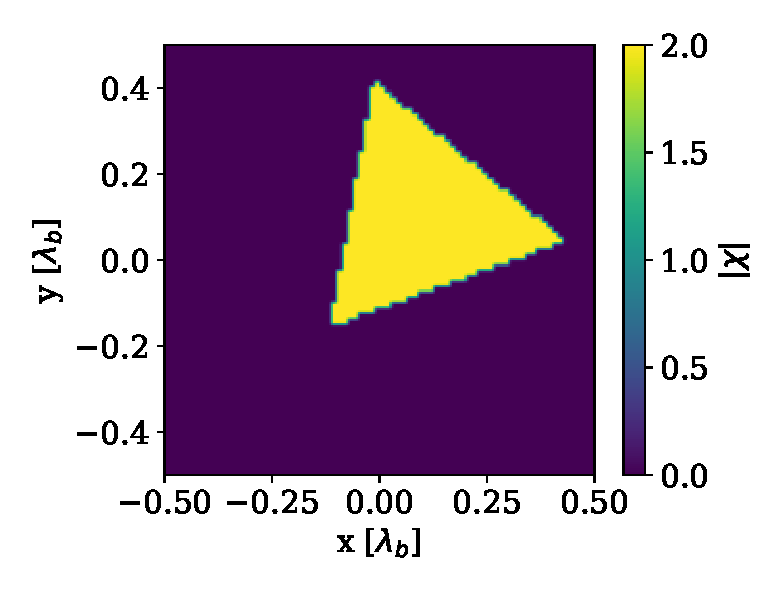
\includegraphics[width=.4\textwidth]{./figuras/transformation_original}} \hspace{.05\textwidth}
				\subfloat[]{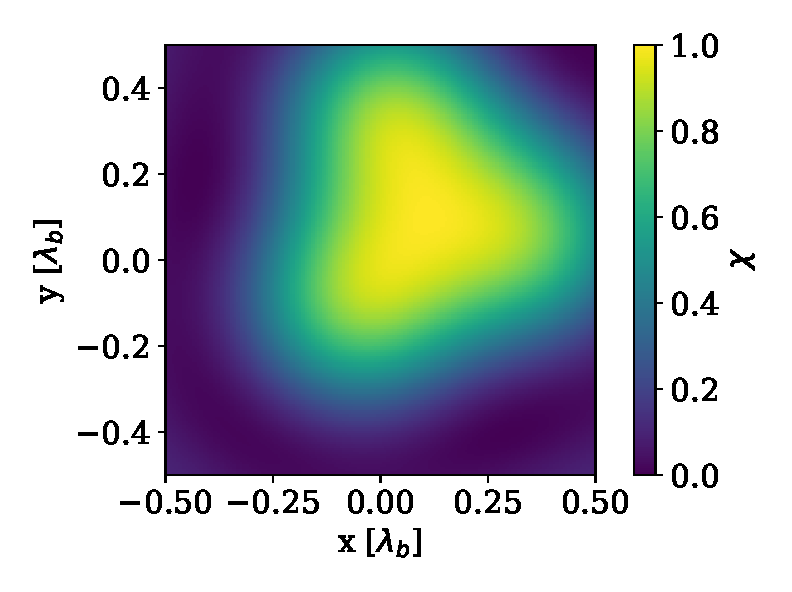
\includegraphics[width=.4\textwidth]{./figuras/transformation_thresholding}} \\
				\subfloat[]{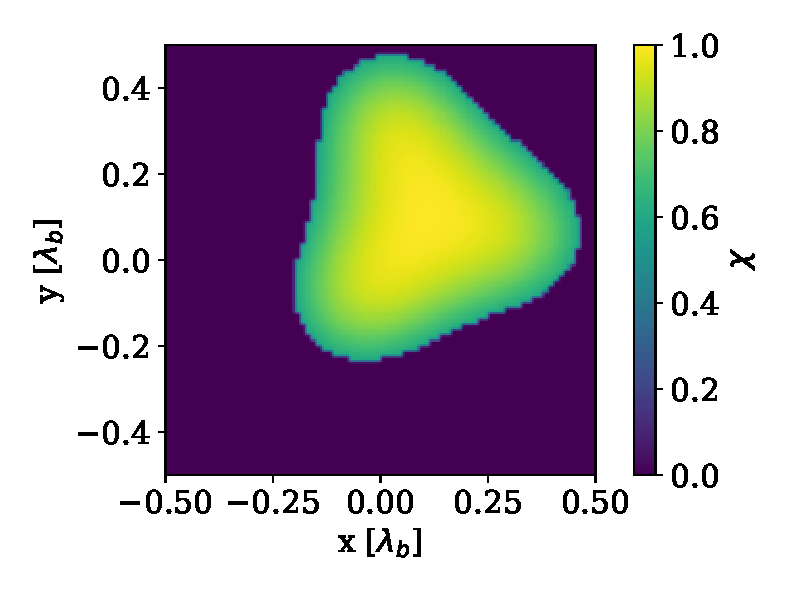
\includegraphics[width=.4\textwidth]{./figuras/transformation_multiplication}} \hspace{.05\textwidth}
				\subfloat[]{\includegraphics[width=.4\textwidth]{./figuras/transformation_final}}
				\caption[Example of the process of transforming a qualitative image into a quantitative one.]{Example of the process of transforming a qualitative image into a quantitative one: (a) ground-truth image; (b) image obtained by OSM ($\boldsymbol{\chi}^{norm}$); (c) image obtained after the thresholding process; and (d) final image obtained after the multiplication step.}
				\label{fig:proposed-methodology:surrogate:optimization:transformation}
			\end{figure}
			
			%The image $\boldsymbol{\chi}$ is also the diagonal elements of the contrast matrix $\boldsymbol{\bar{\chi}}$ in \eqref{eq:3:discretization:collocation:18}. Thus, the data equation error \eqref{eq:3:discretization:collocation:10} might be computed if the total electric field was also evaluated. Therefore, for a given scattered field data and the corresponding Green function matrix, the following bidimensional optimization problem might be defined:'
			The image $\boldsymbol{\chi}$ represents the diagonal elements of the contrast matrix $\boldsymbol{\bar{\chi}}$ mentioned in \eqref{eq:3:discretization:collocation:18}. Consequently, the data equation error \eqref{eq:3:discretization:collocation:10} can be calculated only if the total electric field is evaluated. Hence, a two-dimensional optimization problem can be defined based on a given scattered field data and its corresponding Green function matrix.
			\begin{align}
				T^*, \chi^{F*} =&~\arg\min f(T, \chi^F) \label{eq:proposed-methodology:surrogate:optimization:definition:objfun} \\
				& T\in[0, 1],~ \chi^{F} \in [\chi^F_{min}, \chi^F_{max}] \label{eq:proposed-methodology:surrogate:optimization:definition:bounds} 
			\end{align}
			
			\noindent where $ f(T, \chi^F)$ is the function that determines the data equation error based on the process of solving qualitatively the inverse problem through OSM and applying the transformation according \eqref{eq:proposed-methodology:surrogate:optimization:transformation}. Evidently, the total field must be computed for each pair $(T, \chi^F)$.
			
			%1. Um aspecto importante para qualquer problema de otimização são as características da função objetivo.			
			%2. No problema abordado, enquanto a variação da fator de multiplicação produz variações contínuas no erro da equação de dados, a variação do limiar não produz em pequena escala.
			%3. Uma vez que a imagem é uma representação discreta da função contraste, variações muito pequenas no operador de limiarização podem não causar mudança nenhuma na imagem resultante. Ou seja, se eu variar a variável T de modo que ela não alcance o menor valor de X dentro do objeto, a imagem não muda. Logo, o valor da função objetivo é constante nesse pequeno intervalo.
			Understanding the characteristics of the objective function is crucial for solving any optimization problem effectively. This is because the choice of the most appropriate algorithm depends on this information. Therefore, having knowledge of the objective function's properties is essential for selecting the best optimization method and achieving the desired outcome.
			
			In the optimization problem defined by \eqref{eq:proposed-methodology:surrogate:optimization:definition:objfun}-\eqref{eq:proposed-methodology:surrogate:optimization:definition:bounds}, varying the multiplication factor $\chi^F$ leads to continuous variations in the error of the data equation. However, varying the threshold $T$ does not produce a significant change on a small scale. This is due to the fact that the image is a discrete representation of the contrast function, and small variations in the thresholding operator may not cause any change in the resulting image. Hence, the value of the objective function remains constant in this small interval.
			
			%4. Este efeito ocorre em pequena escala. Ou seja, numa perspectiva macro da função objetivo, ela vai parecer suave e possivelmente até convexa. No entanto, quando se visualizarmos a superfície da função numa escala bem reduzida, notaremos discontinuidades na função. O que permite dizer que a função é multi-escala.
			%5. Isto pode trazer problemas para aplicação de métodos de otimização que se baseiam na informação da derivada. Isto porque a estimativa da derivada se dá pela avaliação da função num local vizinho da solução atual a qual está distante por um valor discreto de uma das variáveis. Logo, o ajuste desse valor discreto para perturbação da solução pode se tornar complicado pois, se o método estiver perto de uma discontinuidade, então o gradiente pode apontar para uma direção errada. Nesses casos, métodos sem-derivadas ou métodos baseados em população podem ser mais eficientes.
			Although this effect occurs on a small scale and the objective function appears smooth and convex from a macro perspective, when we visualize the surface of the function on a smaller scale, we will notice non-smoothness. This makes the function multi-scale and can create problems for optimization methods that depend on derivative information. When close to a roughness, the adjustment of the discrete value for perturbation of the solution might be complicated, making the gradient point in the wrong direction. Derivative-free methods or population-based methods may be more efficient in such cases.
			
			\begin{figure}[!h]
				\centering
				\subfloat[]{\includegraphics[width=.4\textwidth]{./figuras/objfun_groundtruth}\label{fig:proposed-methodology:surrogate:optimization:objfun:groundtruth}} \hspace{.05\textwidth}
				\subfloat[]{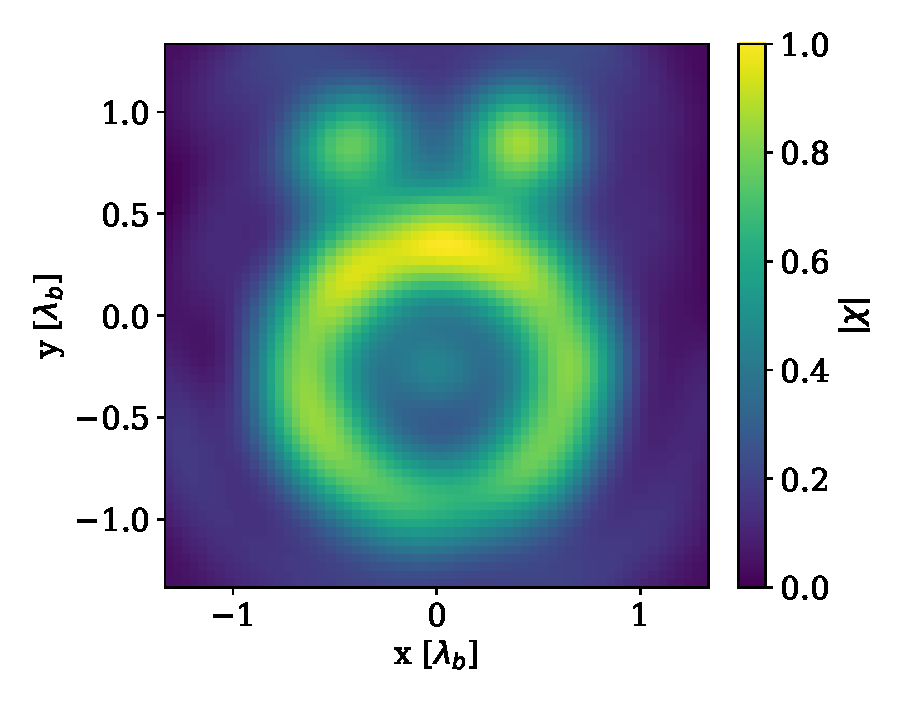
\includegraphics[width=.4\textwidth]{./figuras/objfun_qualitative}\label{fig:proposed-methodology:surrogate:optimization:objfun:qualitative}} \\
				\subfloat[]{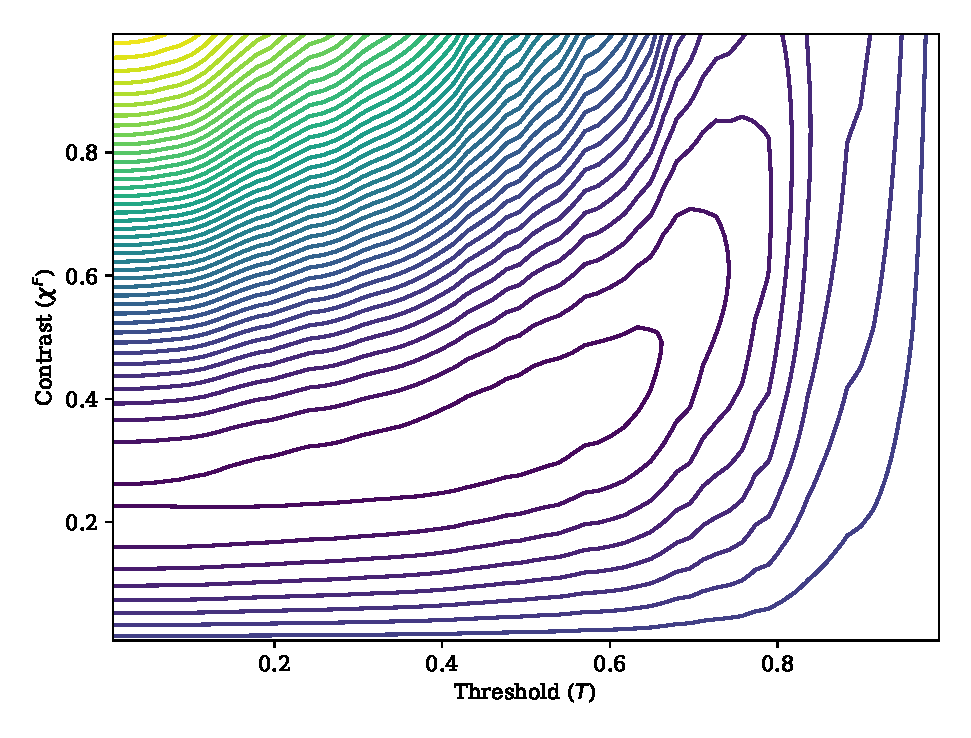
\includegraphics[width=.4\textwidth]{./figuras/objfun_surface}\label{fig:proposed-methodology:surrogate:optimization:objfun:surface}} \hspace{.05\textwidth}
				\subfloat[]{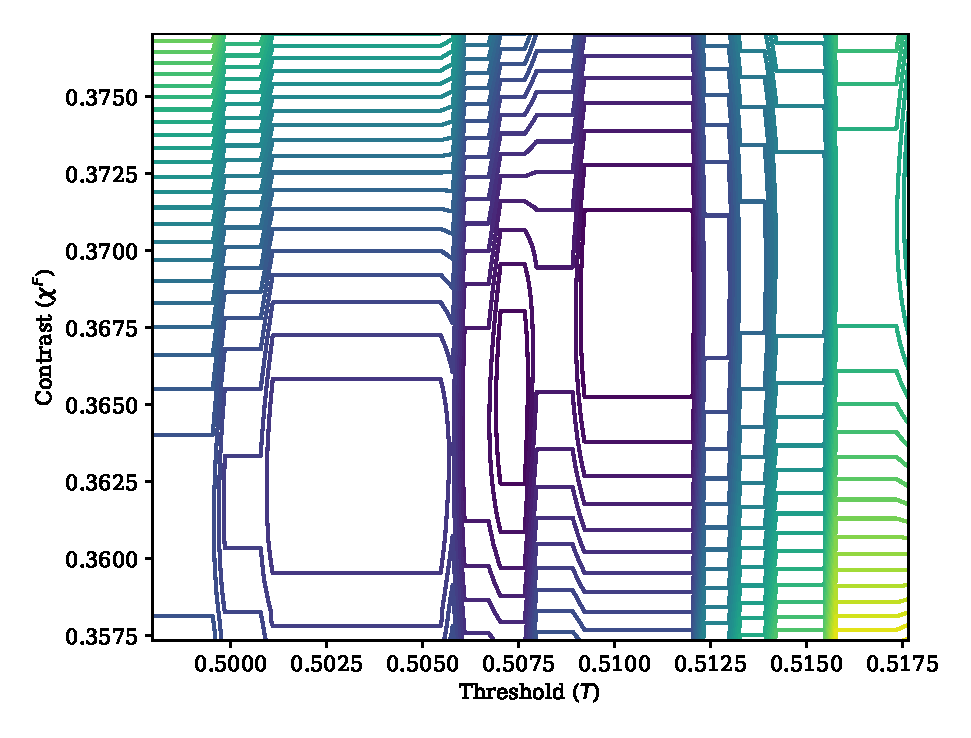
\includegraphics[width=.4\textwidth]{./figuras/objfun_nearoptimum}\label{fig:proposed-methodology:surrogate:optimization:objfun:nearoptimum}}
				\caption[Example of an objective function resulting from the transformation of the inversion problem into a two-dimensional optimization one.]{Example of an objective function resulting from the transformation of the inversion problem into a two-dimensional optimization one: (a) the ground-truth image; (b) the image obtained by OSM; (c) the surface obtained by the transformation of the inversion problem into a two-dimensional optimization one; and (d) a zoom over the region close to the optimum.}
				\label{fig:proposed-methodology:surrogate:optimization:objfun}
			\end{figure}
			
			%6. A figura 4 ilustra este problema. A figura 4(b) mostra a reconstrução a partir do método qualitativo para um teste representado pela figura 4(a). Na figura 4(c) vemos a superfície da função objetivo resultante da transformação do problema de inversão em um problema de otimização bidimensional. Como é possível notar, a superfície, numa perspectiva macro, parece bem suave. No entanto, quando ampliamos a imagem para perto do ótimo (figura 4(d)), vemos as discontinuidades no eixo da variável T.
			Figure \ref{fig:proposed-methodology:surrogate:optimization:objfun} illustrates this problem. Figure \ref{fig:proposed-methodology:surrogate:optimization:objfun:qualitative} shows the reconstruction from the qualitative method for a test represented by Figure \ref{fig:proposed-methodology:surrogate:optimization:objfun:groundtruth}. In Figure \ref{fig:proposed-methodology:surrogate:optimization:objfun:surface}, we see the surface of the objective function resulting from the transformation of the inversion problem into a two-dimensional optimization problem. The surface appears smooth from a macro perspective, but when we zoom in on the image close to the optimum (Figure \ref{fig:proposed-methodology:surrogate:optimization:objfun:nearoptimum}), we see the roughness on the $T$ variable axis.
			
			%7. Outra questão é que o valor ótimo do fator de multiplicação pode não coincidir com o valor exato do contraste da imagem, principalmente em casos de espalhadores homogêneos. Isto porque as variações de contraste dentro da região do objeto impossibilitam reconstruir com exatidão a imagem. Isto é possível obser pela figura 4(d). Uma alternativa para mitigar este efeito é assumir que o objeto é todo homogêneo e truncar os valores dentro da região do objeto pelo seu valor médio ou máximo.
			Another issue is that the optimal value of the multiplication factor may not coincide with the exact value of the image contrast, mainly in cases of homogeneous scatterers. This is because contrast variations within the object region make it difficult to accurately reconstruct the image. An alternative to mitigate this effect is to assume that the object is all homogeneous and truncate the values within the object's region by their average or maximum value.
			
			%8. Por fim, vale à pena frisar que a avaliação da função objetivo não é barata, uma vez que esta depende da execução do resolvedor direto para estimar o campo total correspondente. Logo, pode ser proibitivo a aplicação de um algoritmo de otimização que dependa de muitas avaliações.
			Finally, it is worth emphasizing that the evaluation of the objective function is not cheap since it depends on the execution of the direct resolver to estimate the corresponding total field. Therefore, applying an optimization algorithm that depends on many evaluations can be prohibitive.

		\subsection{Surrogate Models}\label{chap:proposed-methodology:surrogate:explanation}
			
			In many optimization problems, the objective function can be computationally expensive to evaluate, meaning that it takes a long time to compute the value of the function for a given set of input parameters. This can make it difficult to find good quality solutions, as it may take many iterations of the optimization algorithm to explore the search space thoroughly.
			
			Surrogate Models are approximations of the expensive objective function that are designed to reduce the computational cost of evaluating the objective function \citep{schonlau1997computer,mendes2013surrogate,sacks1989design}. A surrogate model is typically trained on a set of input-output pairs, where the inputs are the parameters of the optimization problem and the outputs are the value of the objective function for those parameters. The surrogate model learns to approximate the objective function using this training data, allowing it to make predictions about the value of the objective function for new sets of input parameters without actually evaluating the expensive objective function.
			
			Surrogate models can be used to speed up the convergence of optimization algorithms, as the surrogate model can be evaluated much more quickly than the expensive objective function. This means that the optimization algorithm can explore the search space more quickly, potentially finding good quality solutions in fewer iterations. Additionally, the use of surrogate models can reduce the number of evaluations of the expensive objective function, which can be a significant computational cost in some problems \citep{sobester2008engineering}.
			
			There are many different types of surrogate models, including regression models, neural networks, and Gaussian processes, among others. In this thesis, the Kriging model is considered since it is widely used in optimization problems \citep{emmerich2006single,zhao2011metamodeling,yang2019two} and it has shown slightly better performance in single-objective optimization problems \citep{valadao2020comparative}. 
			
			% The choice of surrogate model will depend on the specific problem and the available data. In some cases, it may be necessary to use multiple surrogate models or to combine surrogate models with other optimization techniques in order to achieve the best results.
		
		\subsection{Kriging Model}\label{chap:proposed-methodology:surrogate:kriging}
		
			Let $y : \mathbb{X} \subset \mathbb{R}^n \Rightarrow \mathbb{R}$ be an objective function for a given problem. A sample with $N$ solutions and their respective evaluations are $\mathbf{X} =  [\mathbf{x}^1, \cdots, \mathbf{x}^N]^T$ and $\mathbf{y} = [y(\mathbf{x}^1), \cdots, y(\mathbf{x}^N)]^T$, respectively. The Kriging model is a regression model where each observation of the objective function is treated as \citep{sacks1989design,schonlau1997computer,jones1998efficient}:
			\begin{equation}
				y(\mathbf{x}^i) = f(\mathbf{x}^i) + e(\mathbf{x}^i),~ i = 1, \cdots, N \label{eq:kriging:responsemodel}
			\end{equation}
		
			\noindent where $f(\mathbf{x}^i) = \mathbf{f}^T\boldsymbol{\alpha} = \sum\limits_{k=0}^d \alpha_kf_k(\mathbf{x}^i)$, $d\le N-1$, is a linear combination of the regression functions $f_k(\cdot)$ and $\alpha_k$, $k=0,\cdots,d$, are the corresponding coefficients; $e(\cdot)$ is a random normal variable with zero mean and variance $\Sigma^2$. Regression functions are similar to the trial functions presented in Section \ref{chap:methods:discretization}. In the scope of present subsection:
			\begin{equation}
				f_k(\mathbf{x}) = \prod\limits_{r=1}^n x_r^{q_r},~ q_r \in [0, Q],~ \sum\limits_{r=1}^n q_r \le Q \label{eq:kriging:trialfunctions}
			\end{equation}

			\noindent where $Q$ is the highest integer that satisfies $\frac{(n+Q)!}{Q!n!} < N-1$ \citep{zhao2011metamodeling}. The covariance of $e(\cdot)$ is assumed as:
			\begin{equation}
				Cov(e(\mathbf{x}^i), e(\mathbf{x}^j)) = \Sigma^2R(\boldsymbol{\theta},\mathbf{x}^i,\mathbf{x}^j) \label{eq:kriging:covariance}
			\end{equation}
		
			\noindent where $R(\cdot, \cdot, \cdot)$ is a Gaussian correlation function whose form is:
			\begin{equation}
				R(\boldsymbol{\theta},\mathbf{x}^i,\mathbf{x}^j) = \prod\limits_{r=1}^n e^{-\theta_r|x_r^i-x_r^j|^2} \label{eq:kriging:gaussiancorrelation}
			\end{equation}
		
			\noindent with $\boldsymbol{\theta} \in \mathbb{H}$, $\mathbb{H} = \left\{[\theta_1,\cdots,\theta_n]|\theta_r>0\forall r=1,\cdots,n\right\}$. Other correlation functions are also possible \citep{sacks1989design,mackay1998introduction}. However, \eqref{eq:kriging:gaussiancorrelation} is often used when the Kriging model is considered \citep{jin2005comprehensive,zhao2011metamodeling}. The parameters $\boldsymbol{\theta}$ are estimated based on the available sample and they mean the importance of each variable and how correlated they are.
			
			The optimal choice of $\boldsymbol{\theta}$, based on the sample data, is defined as the maximum likelihood estimator (MLE), where the likelihood funnction has the following form:
			\begin{equation}
				L(\boldsymbol{\theta}) = \frac{1}{\sqrt{(2\pi\Sigma^2)^N|\mathbf{R}|}}\mathrm{exp}\left(-\frac{1}{2\Sigma^2}(\mathbf{y}-\mathbf{F}\boldsymbol{\alpha})^T\mathbf{R}^{-1}(\mathbf{y}-\mathbf{F}\boldsymbol{\alpha})\right) \label{eq:kriging:mle}
			\end{equation}
		
			\noindent where $\mathbf{F}=[f_k(\mathbf{x}^i)]_{N\times(d+1)}$ and $\mathbf{R} = [R(\boldsymbol{\theta},\mathbf{x}^i,\mathbf{x}^j)]_{N\times N}$ are the regression and correlation matrices, respectively, with $i,j\in {1,\cdots, N}$ and $k\in {0,\cdots,d}$. For a given $\boldsymbol{\theta}$, the expressions:
			\begin{eqnarray}
				\boldsymbol{\hat{\alpha}} &=& \left(\mathbf{F}^T\mathbf{R}^{-1}\mathbf{F}\right)^{-1}\mathbf{F}^T\mathbf{R}^{-1}\mathbf{y} \label{eq:kriging:alphamle} \\
				\hat{\Sigma}^2 = \frac{1}{N} \left(\mathbf{y}-\mathbf{F}\boldsymbol{\hat{\alpha}}\right)^T\mathbf{R}^{-1}(\mathbf{y}-\mathbf{F}\boldsymbol{\hat{\alpha}}) \label{eq:kriging:sigma2mle}
			\end{eqnarray}
		
			\noindent provide the respective MLEs of $\boldsymbol{\alpha}$ and $\Sigma^2$. If \eqref{eq:kriging:alphamle} and \eqref{eq:kriging:sigma2mle} are used in \eqref{eq:kriging:mle}, then the optimal $\boldsymbol{\theta}$ is obtained through:
			\begin{equation}
				\arg\max\limits_{\boldsymbol{\theta}\in \mathbb{H}} \ln~L(\boldsymbol{\theta}) \label{eq:kriging:optimization}
			\end{equation}
		
			\noindent where:
			\begin{equation}
				\ln~L(\boldsymbol{\theta}) = -\frac{N}{2}\ln(2\pi) - N\ln(\hat{\Sigma}) - \ln(|\mathbf{R}|) - \frac{1}{2}
			\end{equation}
		
			By determining the optimal $\boldsymbol{\theta}$ through \eqref{eq:kriging:optimization}, the correlation matrix $\mathbf{R}$ is obtained and $\boldsymbol{\hat{\alpha}}$ and $\hat{\Sigma}^2$ are computed according to \eqref{eq:kriging:alphamle} and \eqref{eq:kriging:sigma2mle}, respectively. Then, for an untried input $\mathbf{x}$, the predicted evaluation and its mean squared error are, respectively:
			\begin{eqnarray}
				\hat{y}(\mathbf{x}) &=& \mathbf{f}^T\boldsymbol{\hat{\alpha}} + \mathbf{r}^T\mathbf{R}^{-1}(y-\mathbf{F}\boldsymbol{\hat{\alpha}}) \label{eq:kriging:prediction} \\
				\hat{s}^2(\mathbf{x}) &=& \hat{\Sigma}^2\left[1-\left(\mathbf{f}^T(\mathbf{x})+\mathbf{r}^T(\mathbf{x})\right) \begin{pmatrix} \mathbf{0} & \mathbf{F}^T \\ \mathbf{F} & \mathbf{R} \end{pmatrix}^{-1} \begin{pmatrix} \mathbf{f}(\mathbf{x}) \\ \mathbf{r}(\mathbf{x}) \end{pmatrix} \right]
			\end{eqnarray}
		
			\noindent where $\mathbf{r}^T(\mathbf{x}) = \left[R(\boldsymbol{\theta}, \mathbf{x}^1, \mathbf{x}), \cdots, R(\boldsymbol{\theta}, \mathbf{x}^N, \mathbf{x})\right]$ is the vector of correlation; $R(\boldsymbol{\theta}, \mathbf{x}^i, \mathbf{x})$ represents the correlation between $e(\cdot)$ at the sampled point $\mathbf{x}^i$ and $e(\cdot)$ at an untried $\mathbf{x}$, for $i=1,\cdots,N$. 
			
			Finally, such Kriging model is an interpolation model. Interestingly, when \eqref{eq:kriging:prediction} is evaluated at a point that belongs to the sample, then the prediction is the actual evaluation. This is due to the matching of $\mathbf{r}^T$ for the considered point with a line of the matrix $\mathbf{R}$.

		\subsection{Surrogate model-Assisted Algorithms}\label{chap:proposed-methodology:surrogate:algorithms}
		
			% 1. Na subseção 3.1, foi visto que a função-objetivo resultante da transformação do problema inversão em um de otimização bidimensional, além de ser multi-escala, é também cara computacionalmente. Estas características decorrem da não-suavidade do operador de limiarização e da necessidade de solução do problema direto para estimativa do erro.
			% 2. Uma alternativa para esses dois problemas é a substituição da função objetivo por um modelo substituto. Tendo em vista que o modelo substituto é um operador de interpolação, ele pode contornar o problema da micro-escala. Ou seja, reconstruir a função-objetivo pelas suas características macroscópicas através de um conjunto de pontos na superfície que não são muito próximos. O modelo substituto será uma função suave desde que use funções de base suaves. Além disso, a predição da avaliação da função objetivo é um processo muito mais barato do que a avaliação em si. Portanto, fica mais viável a aplicação de algoritmos de direção de busca e de população também.
			
			The chapter presented various aspects related to the proposed optimization problem and the use of surrogate models. Subsection \ref{chap:proposed-methodology:surrogate:optimization} showed how the inversion problem was transformed into a two-dimensional optimization problem. However, the obtained objective function is non-smooth and computationally expensive due to the non-smoothness of the thresholding operator and the need to solve the problem directly to estimate the data equation error. To address these challenges, one alternative is to use a surrogate model, which can reconstruct the objective function by considering its macroscopic characteristics through a set of surface points that are not too close together. The surrogate model works as an interpolation operator and can overcome the microscale problem, resulting in a smooth function when smooth basis functions are used. Additionally, predicting the objective function evaluation is less costly than evaluating it, making it feasible to apply search direction and population-based algorithms.
			
			% 3. De uma maneira geral, um algoritmo assistido por modelos substitutos dependem de, em primeiro lugar, obter uma amostra de pontos no espaço de busca com suas respectivas avaliações. Com essa amostra, o modelo substituto da função objetivo é construído. A partir daí, o processo de busca pode ser iniciado e, simulateamente, o modelo substituto é atualizado a partir de novas soluções encontradas e escolhidas para serem avaliadas pela função objetivo. Portanto, além das diferentes formas de obter o conjunto inicial, é possível explorar diferentes metodologias de busca e de atualização do modelo.
			In order to implement an algorithm assisted by surrogate models, the first step is to obtain a sample of points in the search space along with their respective evaluations. Based on this sample, the surrogate model of the objective function can be constructed. Once the surrogate model is obtained, the search process can begin, and the model can be updated with new solutions that are chosen to be evaluated by the objective function. Thus, in addition to the various methods for obtaining the initial set of points, it is also possible to explore different methodologies for searching and updating the surrogate model.
			
			% 4. Com relação às metodologias de obtenção da amostra inicial de soluções para o modelo substituto, uma forma trivial é a amostragem uniforme do espaço de busca. Ou seja, dados os intervalos das variáveis de decisão, são amostrados pontos equidistantes em cada eixo. No entanto, a abordagem mais tradicional é a Latin Hypercube Sampling (LHS) \cite{iman1981apporach}. It is a statistical method that generates quasi-random sampling distributions. It is widely used in computer experiments due to its simplicity and its projection properties in high-dimensional problems. To construct the LHS design, each variable dimension space is divided into n sections, where n represents the number of sampling points. Then, only one point is placed in each of the sections.
			One way to obtain the initial sample of solutions is through uniform sampling of the search space. This involves sampling equidistant points on each axis within the range of decision variables. However, the more traditional approach is Latin Hypercube Sampling (LHS) \cite{iman1981apporach}, which is a statistical method that generates quasi-random sampling distributions. LHS is widely used in computer experiments due to its simplicity and projection properties in high-dimensional problems. To construct the LHS design, the space of each variable dimension is divided into n sections, where n is the number of sampling points. Only one point is then placed in each section.

			
			% 5. Para ilustrar possíveis diferenças entre esses dois métodos de amostragem, foi simulado um problema de um espalhador de alto contraste (Figura 5a). Note que a função objetivo (Figura 5b)  é multimodal. A amostragem pelo método LHS resulta na superfície da Figura 5c, enquanto a obtida pela amostragem uniforme é apresentada na Figura 5d. Note que, na superfície obtida pelo LHS, existe uma barreira separando a região original do mínimo em duas. Nessa separação, não existe nenhuma amostra. Uma vez que o método LHS é estocástico, então cada amostragem pode resultar numa superfície diferente e regiões importantes podem ficar sem nenhuma amostra. Na amostragem uniforme, também não é garantido que uma região fique sem amostras. Principalmente se o número de amostras for baixo. Mas, com um número razoável de amostras, pode-se chegar a uma superfície com características mais parecidas principalmente quando o problema é bidimensional, como é o caso do exemplo da Figura 5. Portanto, para evitar os aspecto estocástico na amostragem, a metodologia uniforme será adotada sendo necessário escolher sempre um número adequado de amostras.
			To illustrate the differences between these two sampling methods, a high-contrast scatterer problem was simulated (Figure \ref{fig:proposed-methodology:surrogate:algorithms:samplings:groundtruth}), resulting in a multimodal objective function (Figure \ref{fig:proposed-methodology:surrogate:algorithms:samplings:objfun}. Sampling by the LHS method resulted in a surface with a barrier separating the original minimum region in two, in which there was no sample (Figure \ref{fig:proposed-methodology:surrogate:algorithms:samplings:objfun}). Since the LHS method is stochastic, each sampling can result in a different surface, and important regions can be left without any samples. Uniform sampling can also result in regions running out of samples, especially if the number of samples is low. However, with a reasonable number of samples, a surface with similar characteristics can be obtained, especially in two-dimensional problems, as it is shown in Figure \ref{fig:proposed-methodology:surrogate:algorithms:samplings:uniform}. Therefore, to avoid the stochastic aspect of sampling, a uniform methodology is adopted, and it is always necessary to choose an adequate number of samples.

			\begin{figure}[!h]
				\centering
				\subfloat[]{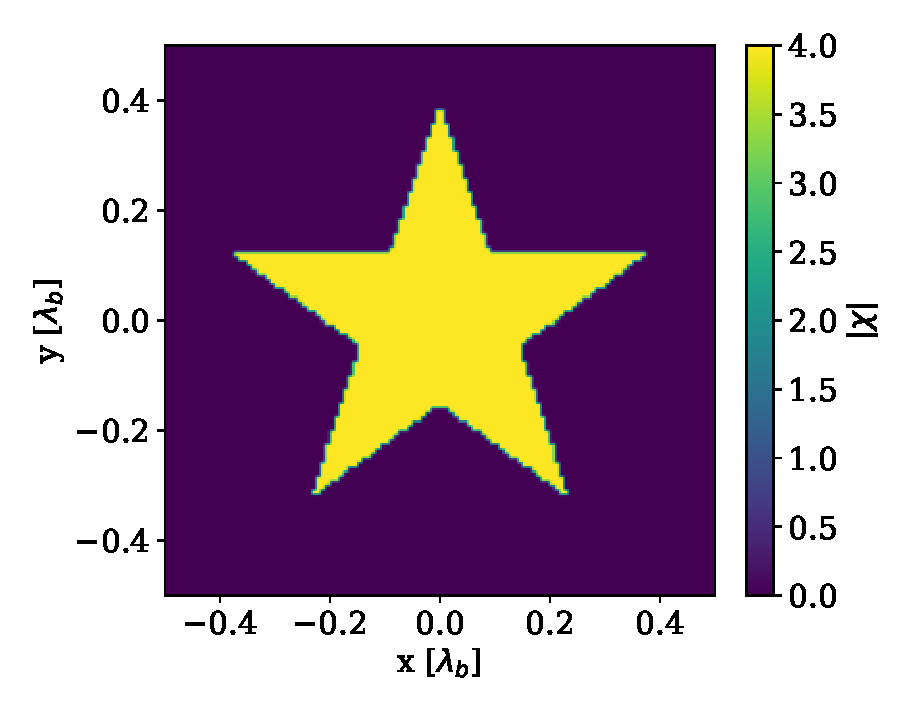
\includegraphics[width=.4\textwidth]{./figuras/samplings_groundtruth}\label{fig:proposed-methodology:surrogate:algorithms:samplings:groundtruth}} \hspace{.1\textwidth}
				\subfloat[]{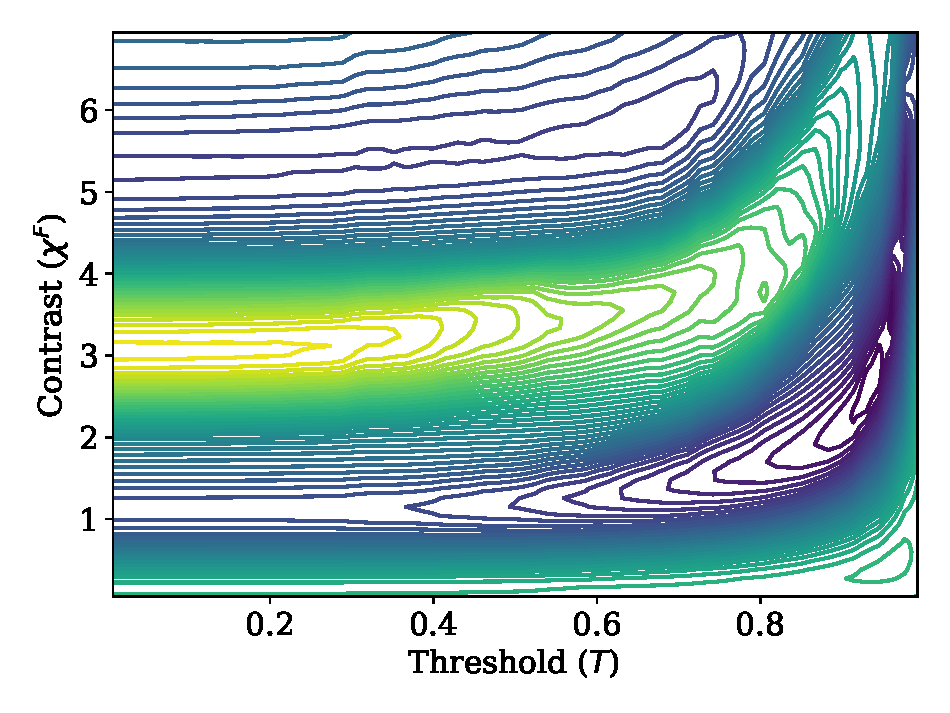
\includegraphics[width=.4\textwidth]{./figuras/samplings_objfun}\label{fig:proposed-methodology:surrogate:algorithms:samplings:objfun}} \\
				\subfloat[]{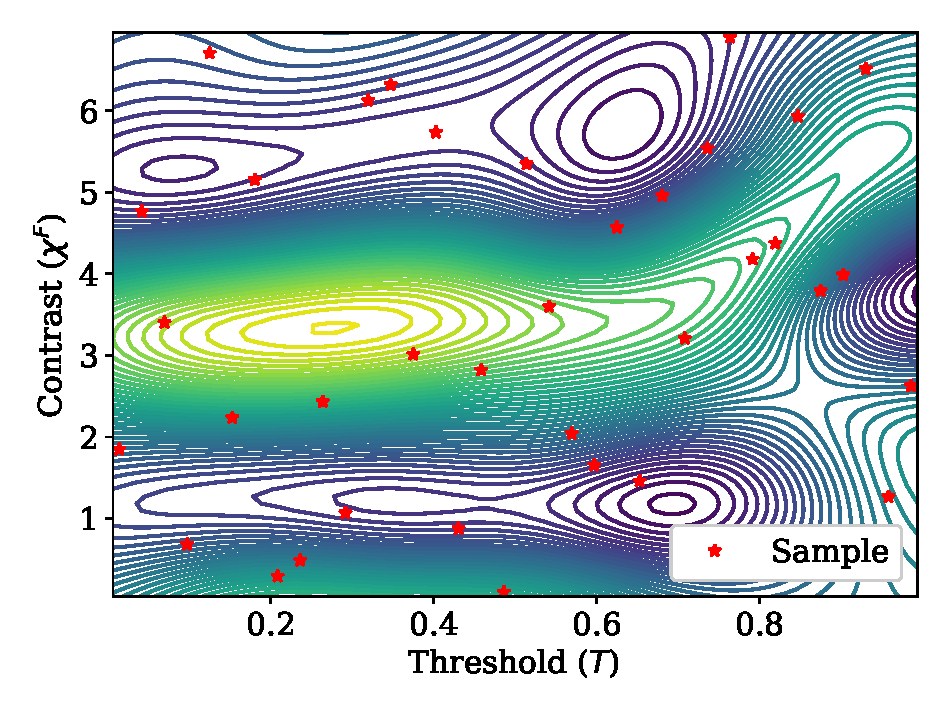
\includegraphics[width=.4\textwidth]{./figuras/samplings_lhs}\label{fig:proposed-methodology:surrogate:algorithms:samplings:lhs}} \hspace{.1\textwidth}
				\subfloat[]{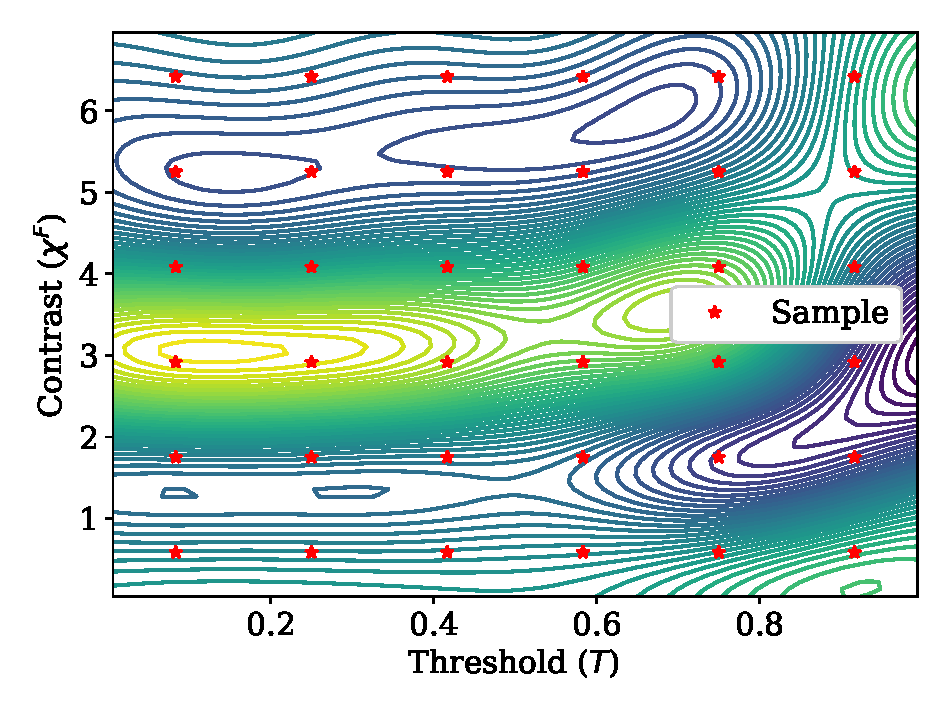
\includegraphics[width=.4\textwidth]{./figuras/samplings_uniform}\label{fig:proposed-methodology:surrogate:algorithms:samplings:uniform}}
				\caption[Comparison of Latin Hypercube Sampling and Uniform Sampling methods for strong scatterer instance.]{Comparison of Latin Hypercube Sampling and Uniform Sampling methods for strong scatterer instance: (a) the ground-truth image; (b) the surface of the corresponding objective-function; (c) the predicted surface obtained by LHS; (d) the predicted surface obtained by uniform sampling.}
				\label{fig:proposed-methodology:surrogate:algorithms:samplings}
			\end{figure}
			
			Surrogate Model-Assisted Evolutionary Algorithms (SAEAs) are a popular approach  \citep{emmerich2006single,liu2014gaussian}. Despite the various possible formulations of SAEAs \citep{buche2005accelerating}, they all share the same general structure \citep{he2023review}. In Figure \ref{fig:proposed-methodology:surrogate:algorithms:saeaflowchart}, the general flowchart is illustrated. The main cycle of the algorithm is initiated after the initial set of solutions is obtained and the surrogate model is built. In each generation of the cycle, the current surrogate-model is utilized to evaluate the fitness values of individuals instead of the real objective-function. An evolutionary algorithm is then employed to continually search for the optimal solution of the problem. Meanwhile, high-quality individuals are selected to update the sample and, therefore, are evaluated according the true objective function to update the surrogate-model \citep{zhou2007combining,liu2014gaussian,sun2017surrogate}. These operations are repeated until the termination condition is met \citep{jin2005comprehensive}.
			
			\begin{figure}[!h]
				\centering
				\includegraphics[width=.8\textwidth]{./figuras/saeaflowchart}
				\caption[The basic flowchart of SAEAs.]{The basic flowchart of SAEAs.}
				\label{fig:proposed-methodology:surrogate:algorithms:saeaflowchart}
			\end{figure}
			
			In surrogate model-assisted optimization algorithms, it is not only population-based algorithms that can be used. Since the surrogate model is constructed from smooth basis functions, it is also possible to use search direction methods based on derivatives. Once the surrogate model is built, a local optimum of the predicted surface can be obtained by applying such methods to a given starting point. This local optimum is then evaluated based on the true objective function, and the surrogate model is updated with this new sample. This process is then repeated with the final solution from the previous iteration as the new starting point. Given that the objective function is reasonably sampled early on, such a method could converge to the optimum solution. A stopping criterion for this method could be consecutive iterations in which the optimal solution does not change. Different formulations can be explored for choosing the first starting point of the search direction method. This can be especially important in multimodal problems, such as the one addressed in this thesis.
		
			In this thesis, three SAEAs approaches are considered. Their differences are the way in which the population is initialized and the way in which the high-quality individuals are selected for updating the model. In addition, two Surrogate model-Assisted Descent Methods (SADMs) are also proposed. Their main difference is the approach for obtaining an initial solution. The next subsubsections describe all of them.
		
			\subsubsection{SAEA1}\label{chap:proposed-methodology:surrogate:algorithms:saea1}
			
				The first SAEA approach is inspired in \citep{salucci2022learned}. After initializing the surrogate model, the population is initialized by simply sampling random points in the search space following the uniform distribution. Their fitness are computed by the surrogate model prediction. Then, the algorithm executes a single iteration of the chosen evolutionary process. After the new population is selected\footnote{The elitism strategy is considered, i.e., the best solution among the parent and offspring populations is preserved for the next generation.}, the current best solution is compared against the sample. If it differs from all available solutions in the sample, its fitness is updated according to the real objective function and it is added to the sample. The model is trained again and all the individuals in the current population are re-evaluated according the updated surrogate model. The cycle repeats and this process continues until the stop criterion is met, at which point the algorithm returns the best solution in the sample. The pseudo-code presented in Algorithm \ref{alg:saea1} outlines this process.
				
				Overall, the following observations are drawn for the considered algorithm:
				\begin{itemize}
					\item The sample contains the initial solution and the best individuals discovered throughout the generations.
					\item The total number of evaluations of the true objective function is not greater than the sum of the number of initial samples and the number of generations.
					\item The offspring population is created using the DE/best/1 operator, and the F factor is randomly selected from a predetermined range.
					\item In addition, a local search step based on a Descent Method is added and performed after a fixed number of generations, which distinguishes this process from the one proposed by \cite{salucci2022learned}.
				\end{itemize}
				
				\begin{algorithm}[!h]
					\caption[Explanation of the functioning of the SAEA1 algorithm.]{The SAEA1 algorithm.}
					\label{alg:saea1}
					\KwIn{Scattered field data, discretization configuration, lower and upper bounds for $\chi^F$ and $T$, number of initial sampled solutions, population size}
					\KwOut{Contrast image.}
					Solve qualitatively the problem and obtain the normalized contrast image.\\
					Sample solutions within the search space uniformly in the defined interval of $\chi^F$ and $T$.
					Evaluate the sampled solutions.\\
					Evaluations $\leftarrow$ number of initial sampled solutions.\\
					Build and train the surrogate model based on the sample.\\
					Initialize a population of individuals by randomizing $\chi^F$ and $T$ values following the uniform distribution.\\
					Set their fitness according to their corresponding prediction obtained by the surrogate model.\\
					\While{stopping criteria is not met}{
						Generate a offspring population based on the DE/best/1 operator.\\
						Evaluate the offspring based on the surrogate model.\\
						Selected the new population considering the union of parents and offspring individuals by Binary Tournament and preserving the best solution among them (elitism).\\
						\If{the local search has not been executed in the last $N_{LS}$ generations}{
							Perform a local search using a Steepest Descent algorithm considering the current best solution as initial guess and the surrogate model as objective function.\\
							\If{the returned solution by the local search is better}{
								Update the current best solution.\\
							}	
						}
						\If{the current best solution is not equal to any other in the sample}{
							Evaluate the current best solution according the objective function.\\
							Evaluations $\leftarrow$ evaluations + 1\\
							Add the current best solution to the sample.\\
							Train the surrogate model.\\
							Re-evaluate the population using the updated surrogate model.\\
						}
					}
				\end{algorithm}
			
			\subsubsection{SAEA2}\label{chap:proposed-methodology:surrogate:algorithms:saea2}
				
				The second approach is inspired in the one proposed by \cite{valadao2020comparative}. The approach for selection and mutation in this algorithm differs from the typical prediction model-based population evaluation implemented in SAEA1. Instead, individual evaluation using the real function serves as the criterion for selection. The mutation strategy is also distinct, with mutation vectors calculated based on solutions stored in an archive. The archive is initially populated with the best solutions from the samples and is updated in each generation with the best $N_A$ solutions from the updated sample. Each offspring-individual is generated from a sub-selection of solutions, generated and evaluated by the surrogate model. The sub-selection generates a set of solutions, and the one with the best value for the prediction of the objective function is selected as the offspring. Then, its fitness is updated according the real objective function. The pseudo-code presented in Algorithm \ref{alg:saea2} outlines this process.
				
				In practice, the described algorithm leads to the following observations:
				\begin{itemize}
					% \item A amostra de soluções é sempre atualizada com as melhores soluções encontradas até geração atual. Logo, soluções com avaliaçõs ruins são retiradas de modo que o modelo prioriza mais a reconstrução da região mais promissora.
					\item The sample solutions are continuously updated with the best solutions found up to the current generation. This means that sampled solutions with the worst evaluations are removed to prioritize the reconstruction of the most promising region.
					% \item A cada geração, o número de avaliações aumenta com o tamanho da população. Portanto, este algoritmo tende a gastar mais avaliações para convergir.
					\item The number of evaluations increases with each generation in proportion to the population size, causing this algorithm to require more evaluations to converge.
					% \item Os mesmos operadores de mutação e de busca local foram aplicados nesta versão do algoritmo.
					\item The current version of the algorithm applies the same mutation and local search operators in each iteration.
				\end{itemize}
    
				\begin{algorithm}[!h]
					\caption[Explanation of the functioning of the SAEA2 algorithm.]{The SAEA2 algorithm.}
					\label{alg:saea2}
					\KwIn{Scattered field data, discretization configuration, lower and upper bounds for $\chi^F$ and $T$, number of initial sampled solutions, population size}
					\KwOut{Contrast image.}
					Solve qualitatively the problem and obtain the normalized contrast image.\\
					Sample solutions within the search space uniformly in the defined interval of $\chi^F$ and $T$.
					Evaluate the sampled solutions.\\
					Evaluations $\leftarrow$ number of initial sampled solutions.\\
					Build and train the surrogate model based on the sample.\\
					Initialize a population of individuals by selecting the $p$ best solutions from the sample.\\
					Store in the archive the best $N_A$ solutions.\\
					\While{stopping criteria is not met}{
						Generate $k$ solutions for each one in the population based on the DE/best/1 operator and evaluate them according to the surrogate model.\\
						For each group of $k$ solutions, selects the best, evaluate it according to the real function and set it as offspring individual.\\
						Evaluations $\leftarrow$ evaluations $+$ population size.\\
						Selected the new population considering the union of parents and offspring individuals by Binary Tournament and preserving the best solution among them (elitism).\\
						\If{the local search has not been executed in the last $N_{LS}$ generations}{
							Perform a local search using a Steepest Descent algorithm considering the current best solution as initial guess and the surrogate model as objective function.\\
							\If{the returned solution by the local search is better}{
								Update the current best solution.\\
							}	
						}
						\If{the current best solution is not equal to any other in the sample}{
							Add the current best solution to the sample.\\
							Train the surrogate model.\\
						}
						Update the archive with the $N_A$ best solutions in the sample.\\
					}
				\end{algorithm}
	
			\subsubsection{SAEA3}\label{chap:proposed-methodology:surrogate:algorithms:saea3}
			
				% A principal vantagem do SAEA1 é gastar somente uma avaliação por geração. Já a principal do SAEA2 é considerar um arquivo de melhores soluções como indivíduos-pais no momento da mutação. Estas duas características podem ser combinadas numa formulação híbrida, a SAEA3, na qual a população de indivíduos pais e filhos continua sendo avaliada pelo modelo substituto, ao passo que os vetores de mutação são gerados considerando um arquivo com as melhores soluções da amostra. Dessa forma, apenas a melhor solução da geração é avaliada pela função real. Desta forma, um número alto de gerações que o SAEA2 pode ser considerado e os indivíduos filhos tendem a herdar mais características das melhores soluções.
				SAEA1 has the main advantage of spending only one evaluation per generation, while SAEA2 has the advantage of considering an archive of best solutions as parents during mutation. The features of these two algorithms can be combined in a hybrid formulation, called SAEA3, where the population of parent and offspring individuals is evaluated by the surrogate model, and mutation vectors are generated based on a file with the best sample solutions. As a result, only the best solution of the generation is evaluated by the actual function. This approach enables SAEA3 to have a high number of generations, similar to SAEA1, while the offspring individuals tend to inherit more characteristics of the best solutions (exploitation), similar to SAEA2. The same mutation and local search operators in each iteration. The pseudo-code presented in Algorithm \ref{alg:saea3} outlines this process.
				
				\begin{algorithm}[!h]
					\caption[The SAEA3 algorithm.]{Explanation of the functioning of the SAEA3 algorithm.}
					\label{alg:saea3}
					\KwIn{Scattered field data, discretization configuration, lower and upper bounds for $\chi^F$ and $T$, number of initial sampled solutions, population size}
					\KwOut{Contrast image.}
					Solve qualitatively the problem and obtain the normalized contrast image.\\
					Sample solutions within the search space uniformly in the defined interval of $\chi^F$ and $T$.
					Evaluate the sampled solutions.\\
					Evaluations $\leftarrow$ number of initial sampled solutions.\\
					Build and train the surrogate model based on the sample.\\
					Initialize a population of individuals by selecting the $p$ best solutions from the sample.\\
					Store in the archive the best $N_A$ solutions.\\
					\While{stopping criteria is not met}{
						Generate $k$ solutions for each one in the population based on the DE/best/1 operator and evaluate them according to the surrogate model.\\
						For each group of $k$ solutions, selects the best and set it as offspring individual.\\
						Selected the new population considering the union of parents and offspring individuals by Binary Tournament and preserving the best solution among them (elitism).\\						
						\If{the local search has not been executed in the last $N_{LS}$ generations}{
							Perform a local search using a Steepest Descent algorithm considering the current best solution as initial guess and the surrogate model as objective function.\\
							\If{the returned solution by the local search is better}{
								Update the current best solution.\\
							}	
						}
						\If{the current best solution is not equal to any other in the sample}{
							Evaluate the current best solution according the objective function.\\
							Evaluations $\leftarrow$ evaluations + 1\\
							Add the current best solution to the sample.\\
							Train the surrogate model.\\
							Re-evaluate the population using the updated surrogate model.\\
						}
						Update the archive with the $N_A$ best solutions in the sample.\\
					}
				\end{algorithm}
			
			\subsubsection{SADM1}\label{chap:proposed-methodology:surrogate:algorithms:sadm1}
			
				% 1. Os algoritmos evolutivos podem explorar todo o espaço de busca, uma vez que são baseados em uma população de soluções.
				% 2. Quando um operador de busca local é aplicado sobre a atual melhor solução, o desempenho pode melhorar uma vez que se realiza uma busca mais intensa sobre uma solução potencial.
				% 3. O processo de amostragem do espaço de busca feito para construir o modelo substituto inicial pode ser pensado como uma população de soluções. Desta forma, se essa amostragem for razoavelmente ampla, a bacia de atração com maior potencial tem boas chances de ser amostrada. Nessas condições, podemos aplicar diferentes estratégias para escolher um ponto inicial e aplicar um algoritmo de direção de busca sobre o modelo substituto.
				% 4. Obviamente, a melhor solução encontrada pode não estar tão próxima do ótimo global. No entanto, esta pode ser avaliada de acordo com a função real e adicionada ao conjunto de amostras para atualizar o modelo.
				% 5. Logo, se esse processo for repetido iterativamente, o algoritmo tenderá a convergir para um local quando a soluções ótimas encontradas em um conjunto de iterações forem idênticas ou muito próximas.
				% 6. A grande questão é então como escolher a solução inicial que vai dar início ao processo iterativo de otimização.
				% 7. Uma possível estratégia é executar um algoritmo evolutivo considerando o modelo substituto inicial e tomar como solução inicial do processo iterativo a melhor solução encontrada pelo algoritmo evolutivo. Assim, uma busca global é feita e o processo iterativo tende a se concentrar na região da melhor bacia de atração disponível na primeira construção do modelo.
				
				Evolutionary algorithms are powerful optimization techniques based on a population of solutions. They are capable of exploring the entire search space (exploration), and when combined with local search operators, performance can improve significantly due to the exploitation of a potential solution. The initial surrogate model construction can be seen as a population of solutions, which, if sampled broadly, can cover the most promising region of the search space. Different strategies can be applied to choose a starting point and apply a steepest descent algorithm on the surrogate model.
				
				The best solution found may not necessarily be close to the global optimum, but it can be evaluated against the actual function and added to the sample set to update the model. By repeating this process iteratively, the algorithm will tend to converge to a location when the optimal solutions found in a set of iterations are identical or very close. However, the question of how to choose the initial solution that will start the iterative optimization process remains.
				
				One possible strategy is to run an evolutionary algorithm considering the initial surrogate model and take the best solution found as the initial solution of the iterative process. This way, a global search is performed, and the iterative process tends to focus on the region of the best basin of attraction available in the first construction of the model. Such an approach will be denoted as SADM1 where the initials stand for Surrogate-model Assisted Descent Method. The pseudo-code presented in Algorithm \ref{alg:sadm1} outlines this process.
				
				Overall, the following observations are drawn for the considered algorithm:
				\begin{itemize}
					\item The evolutionary algorithm employed to determine an initial guess is the Differential Evolution with the following formulation: DE/best/1/bin \citep{rocca2011differential}.
					\item The employed descent method is the L-BFGS-B algorithm which is a limited-memory version of Broyden-Fletcher-Goldfarb-Shanno (BFGS) algorithm for boundary constrained optimization \citep{byrd1995limited,zhu1997algorithm}.
				\end{itemize}
				
				\begin{algorithm}[!h]
					\caption[Explanation of the functioning of the SADM1 algorithm.]{The SADM1 algorithm.}
					\label{alg:sadm1}
					\KwIn{Scattered field data, discretization configuration, lower and upper bounds for $\chi^F$ and $T$, number of initial sampled solutions, population size}
					\KwOut{Contrast image.}
					Solve qualitatively the problem and obtain the normalized contrast image.\\
					Sample solutions within the search space uniformly in the defined interval of $\chi^F$ and $T$.
					Evaluate the sampled solutions.\\
					Evaluations $\leftarrow$ number of initial sampled solutions.\\
					Build and train the surrogate model based on the sample.\\
					Run an evolutionary algorithm considering the surrogate model as objective function and take the best solution as current solution.\\
					Evaluate the current solution according the true objective function, add it to the sample and retrain the model.\\
					\While{stopping criteria is not met}{
						Run the descent method considering the current solution as initial guess and optimizing the predicted surface.\\
						Evaluate the returned solution according the true objective function.\\
						Evaluations $\leftarrow$ evaluations + 1\\
						\If{the returned solution is not equal to any other in the sample}{
							Add the current best solution to the sample.\\
							Train the surrogate model.\\
						}
						\If{the returned solution is better than the current one}{
							Set the current solution as the returned by the last call of the descent optimization.\\
						}
					}
				\end{algorithm}
	
			\subsubsection{SADM2}\label{chap:proposed-methodology:surrogate:algorithms:sadm2}
			
				% 1. Ao invés de determinar o ponto inicial para o processo iterativo do SADM através da utilização de um algoritmo evolucionário, uma alternativa mais simples é escolher a melhor amostra como ponto de partida. Ou seja, após amostrar o espaço de busca, o processo iterativo começa assumindo como solução atual a melhor amostra do modelo.
				% 2. Além de mais simples, uma vantagem é evitar a possibilidade de convergir para uma outra bacia de atração diferente da de mínimo global quando esta estiver perto da melhor amostra. Em outras palavras, considerando a superfície gerada pelo modelo substituto, o algoritmo evolutivo não garante a convergência para o mínimo globa, uma vez que é estocástico. No entanto, se por um acaso o mínimo global estiver próximo da melhor amostra, o que é bem possível, então a primeira iteração do SADM convergirá para esse local.
				% 3. É claro que, se a superfície não for bem amostrada no começo, então poder ser o processo convirja para uma região diferente da do ótimo global da função real. E isso pode ser mais complicado em casos de espalhadores fortes, onde a função objetivo tende a ser multi-modal. Mas quando a função objetivo é menos complexa, então essa estratégia pode ser bem eficiente.
				
				Rather than determining the starting point for the SADM iterative process using an evolutionary algorithm, a simpler alternative is to choose the best sample as the starting point. That is, after sampling the search space, the iterative process starts assuming the best sample of the model as the current solution. In addition to being simpler, an advantage is to avoid the possibility of converging to another basin of attraction different from the global minimum when this is close to the best sample. In other words, considering the surface generated by the surrogate model, the evolutionary algorithm does not guarantee convergence to the global minimum, since it is stochastic. However, if by chance the global minimum is close to the best sample, which is quite possible, then the first iteration of SADM will certainly converge to that location. Of course, if the surface is not sampled well at the beginning, then the process may converge to a region other than the global optimum of the real function. And this can be more complicated in cases of strong scatterers, where the objective function tends to be multi-modal. But when the objective function is less complex then this strategy can be quite efficient. This approach will be denoted as SADM2 and its pseudo-code is shown in Algorithm \ref{alg:sadm2}. The L-BFGS-B algorithm will be used in a similar manner to SADM1.
				
				\begin{algorithm}[!h]
					\caption[Explanation of the functioning of the SADM2 algorithm.]{The SADM2 algorithm.}
					\label{alg:sadm2}
					\KwIn{Scattered field data, discretization configuration, lower and upper bounds for $\chi^F$ and $T$, number of initial sampled solutions, population size}
					\KwOut{Contrast image.}
					Solve qualitatively the problem and obtain the normalized contrast image.\\
					Sample solutions within the search space uniformly in the defined interval of $\chi^F$ and $T$.
					Evaluate the sampled solutions.\\
					Evaluations $\leftarrow$ number of initial sampled solutions.\\
					Build and train the surrogate model based on the sample.\\
					Set the best sample as the current solution.\\
					\While{stopping criteria is not met}{
						Run the descent method considering the current solution as initial guess and optimizing the predicted surface.\\
						Evaluate the returned solution according the true objective function.\\
						Evaluations $\leftarrow$ evaluations + 1\\
						\If{the returned solution is not equal to any other in the sample}{
							Add the current best solution to the sample.\\
							Train the surrogate model.\\
						}
						\If{the returned solution is better than the current one}{
							Set the current solution as the returned by the last call of the descent optimization.\\
						}
					}
				\end{algorithm}
	
	\section{EISPY2D: A Platform for Developing and Testing Algorithms for EISPs}\label{chap:proposed-methodology:library}
		
		This section presents the proposed framework for the development and testing of algorithms for the electromagnetic inverse scattering problem. The framework is a Python package with implemented classes that provide a structured environment for algorithm development and testing. The novelty of the proposed framework lies in three key aspects. Firstly, it includes the collection of indicators with the proposal of two specific metrics that allow for a comprehensive evaluation of the algorithms' performance. Secondly, the framework proposes an approach to test randomization, which ensures a fairer and more reliable comparison between algorithms. Finally, a statistical routine based on traditional statistical tests is proposed to compare the algorithms' performance. This section provides a brief description of the proposed framework and its features, highlighting the significance and contribution of each aspect.
		
		\subsection{Structure Description}\label{chap:proposed-methodology:library:performance}

			%Para poder comparar algoritmos, foi necessário desenvolver uma plataforma comum para as implementações. Esta plataforma foi desenvolvida em forma de uma biblioteca programada na linguagem Python3  \citep{python3}. Com uma estrutura baseada em orientação a objeto, a biblioteca implementa o problema bidimensional com as configurações de domínio definidas da Seção \ref{chap:methods:definition}. Por isso, ela foi batizada como \textit{eispy2d}. O diagrama de classes UML pode ser visualizado na \autoref{fig:4:eispy2d}.
			In order to be able to compare algorithms, it was necessary to develop a common platform for the implementations. This platform was developed as a library programmed in the Python3 language \citep{vanrossum2010python}. With a structure based on object orientation, the library implements the two-dimensional problem with the domain configurations defined in Section \ref{chap:methods:definition}. Therefore, it was named \textit{eispy2d}. The UML class diagram can be seen in \autoref{fig:4:eispy2d}.
			%\begin{figure}[p]
			%	\centering
			%	\hspace*{-1in}
			%	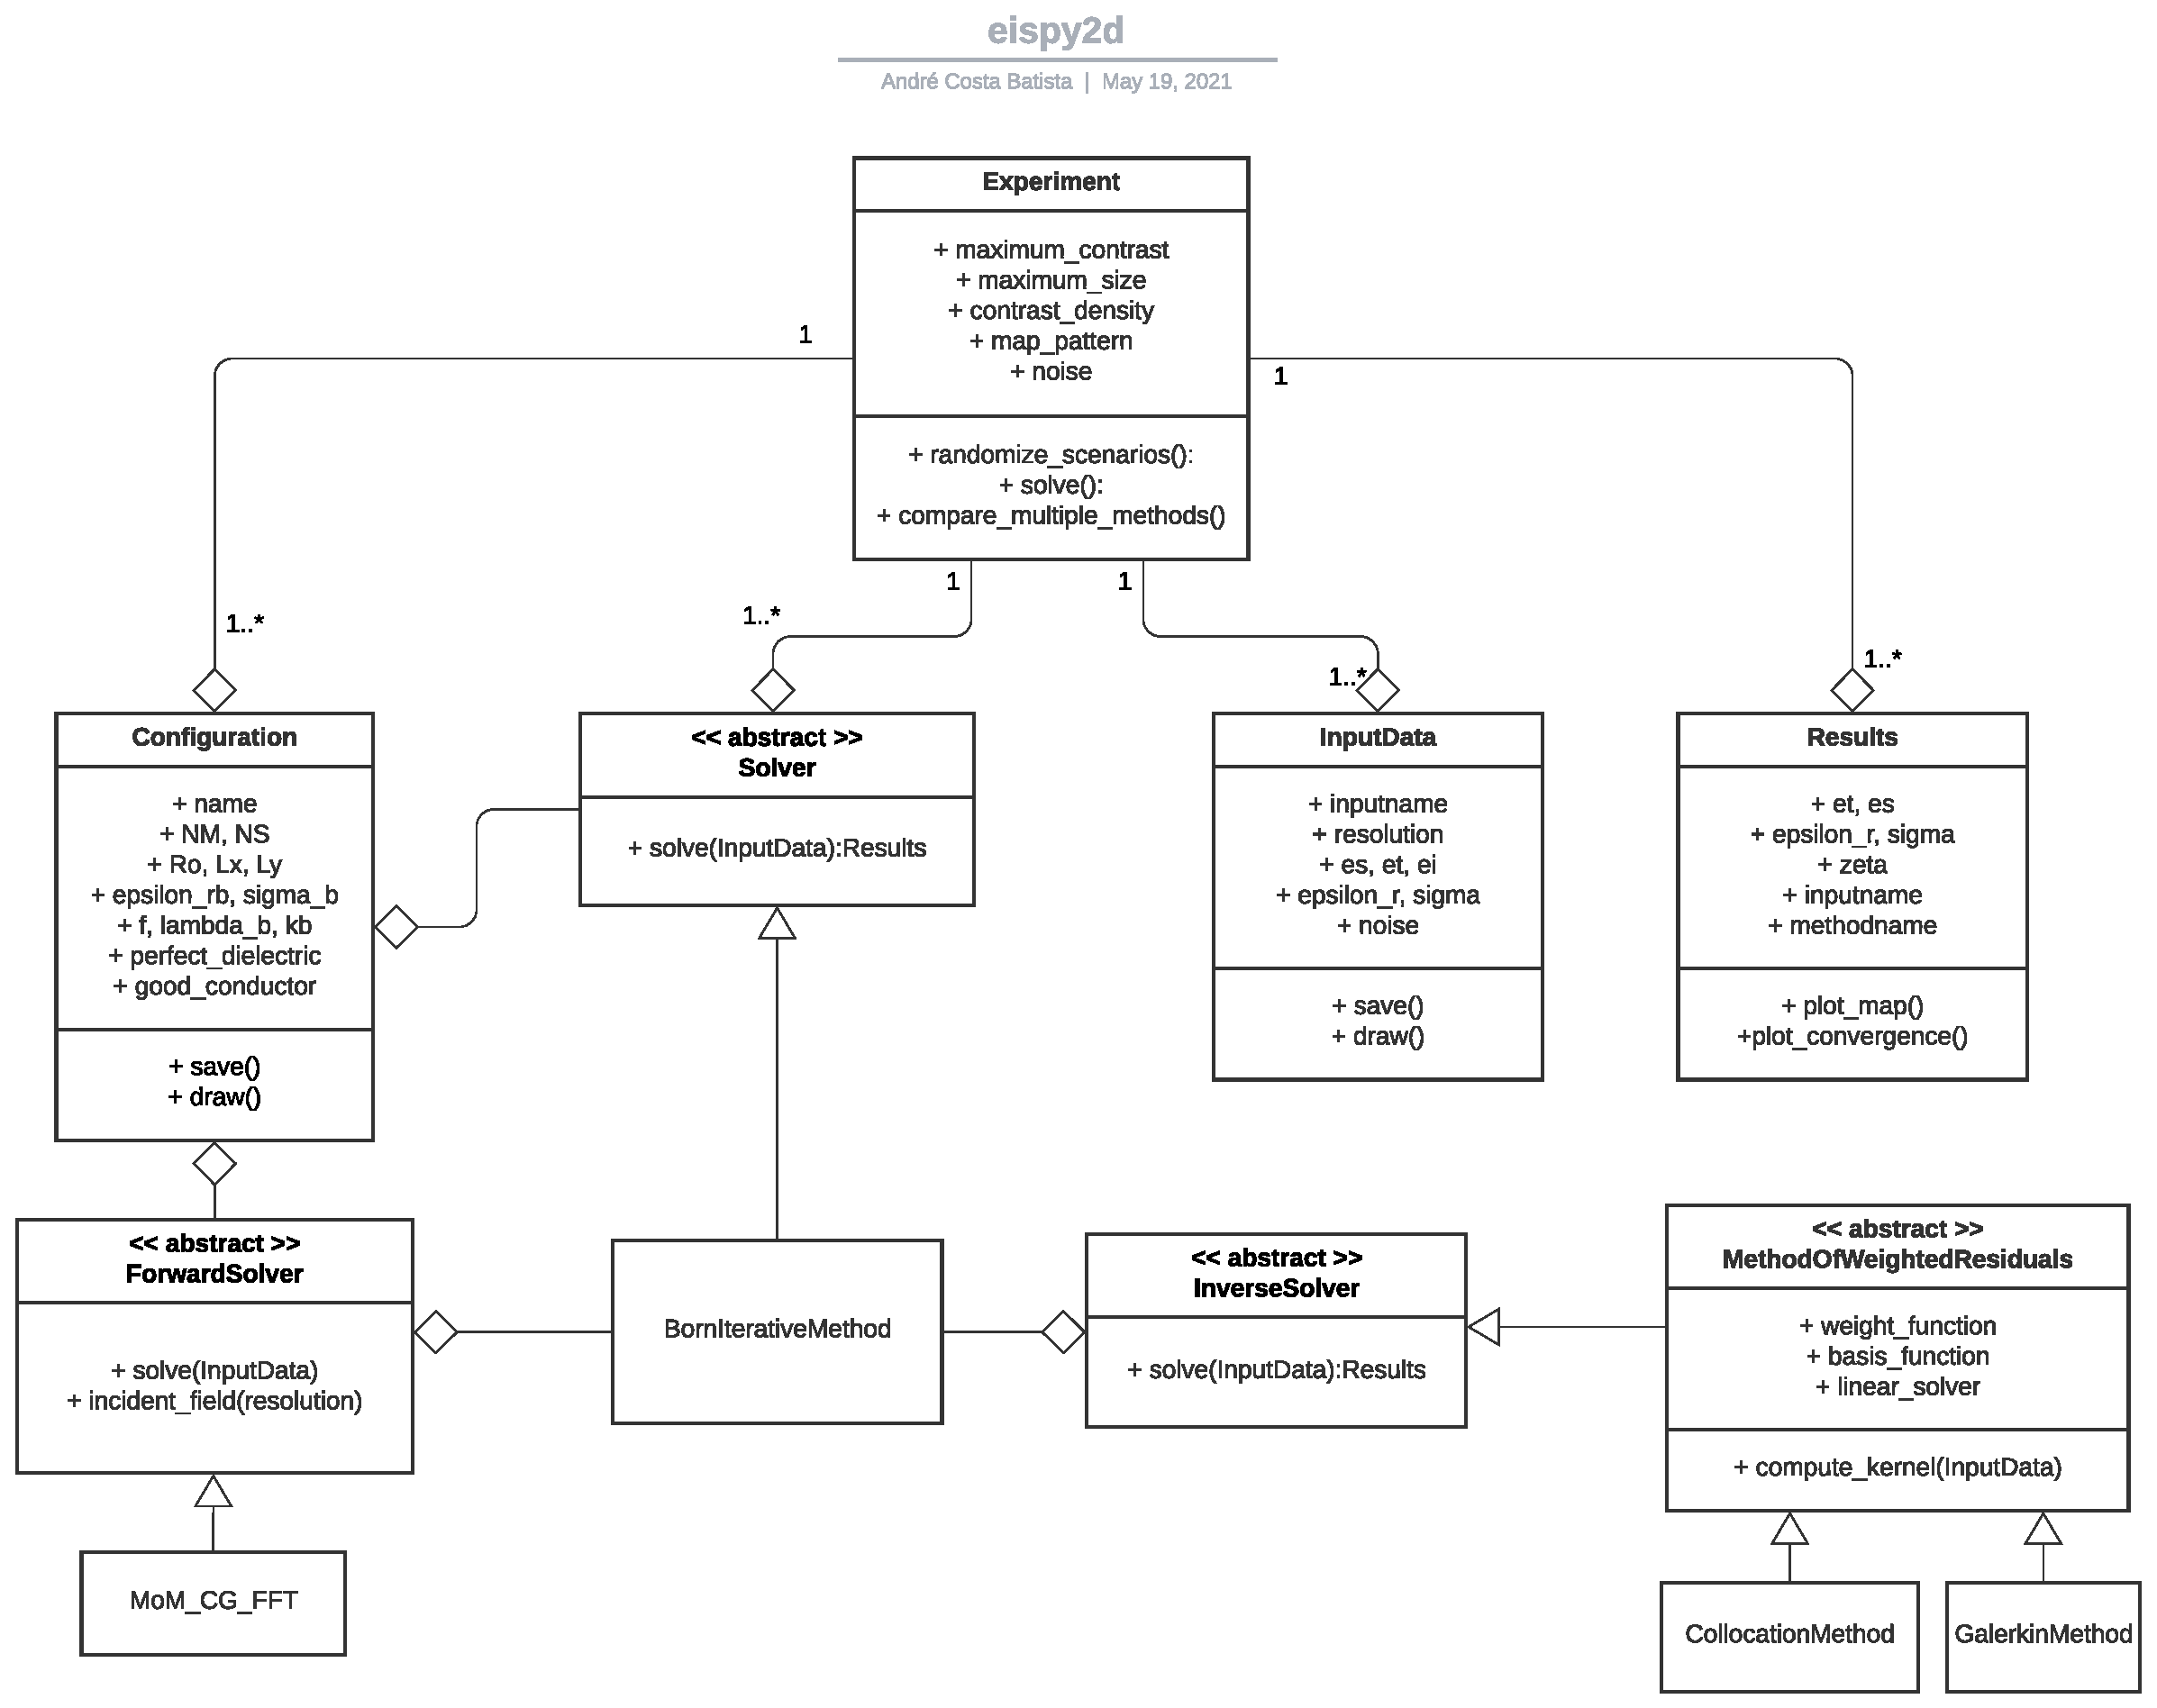
\includegraphics[width=.95\paperwidth, angle=90]{./figuras/eispy2d.eps}
			%	\vspace*{0.2in}
			%	\caption{UML Class Diagram of \textit{eispy2d} library.}
			%	\label{fig:4:eispy2d}
			%\end{figure}
			\begin{figure}[!h]
				\centering
				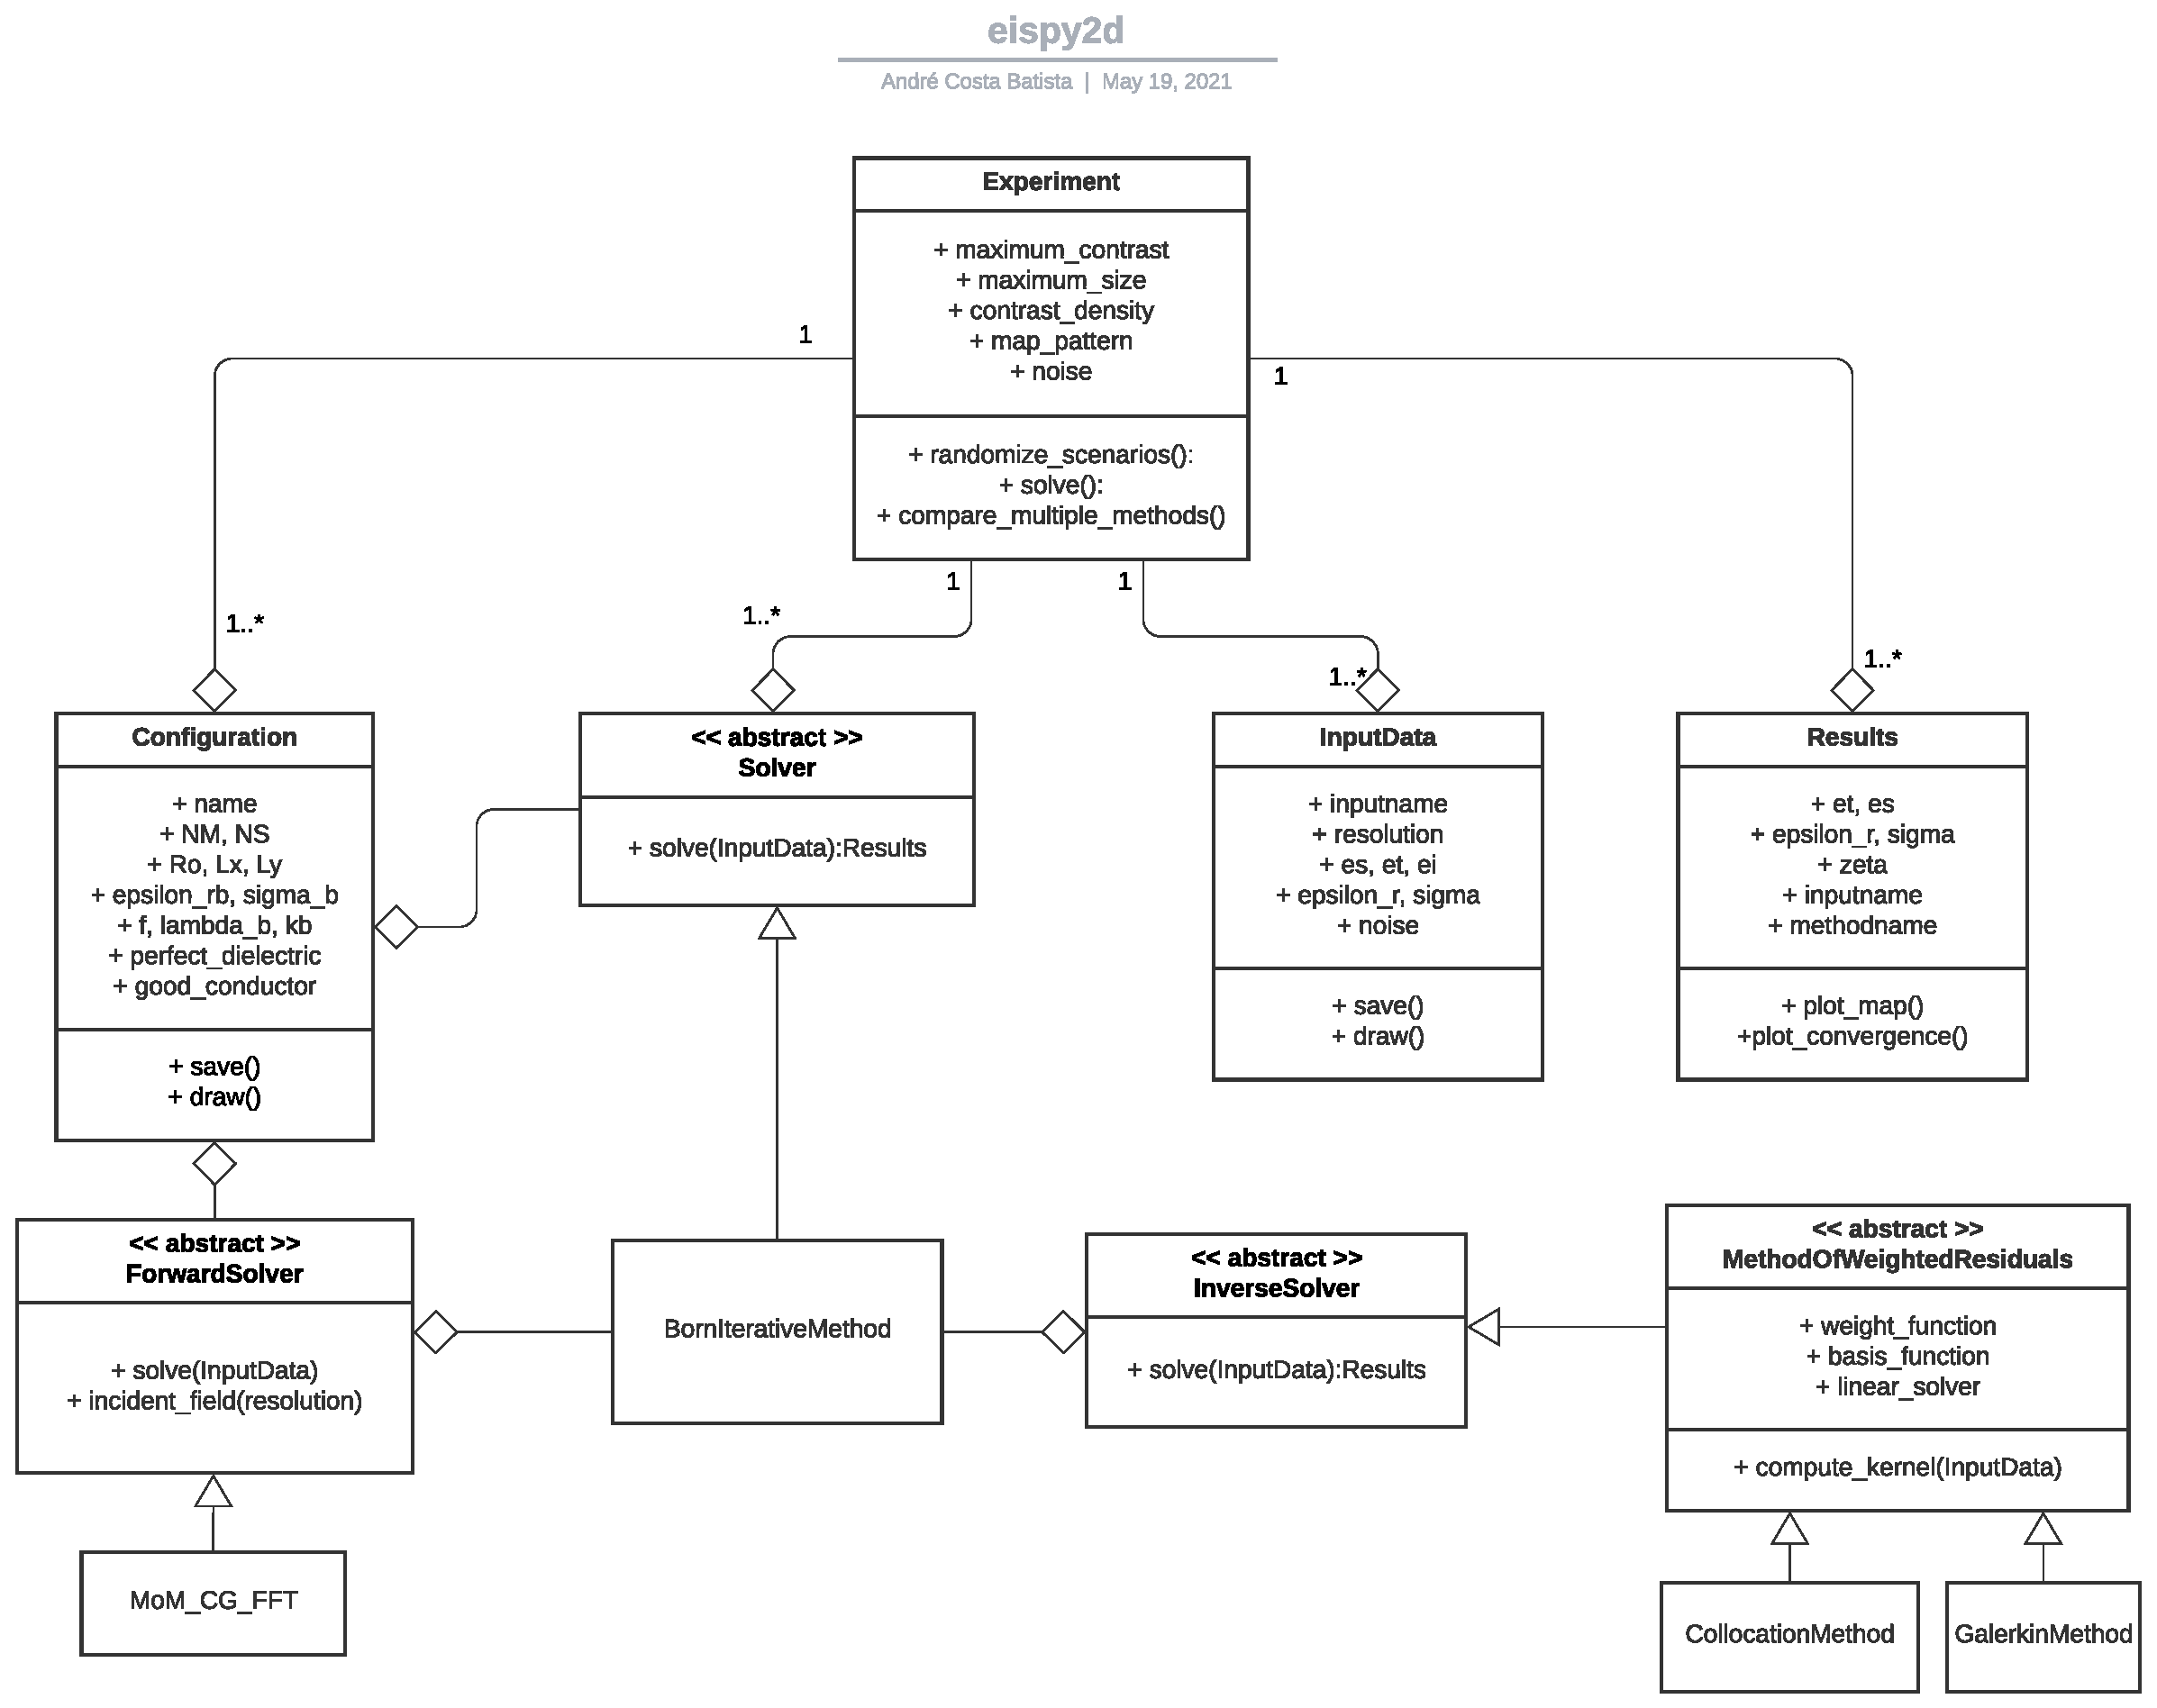
\includegraphics[width=\textwidth]{./figuras/eispy2d.eps}
				\caption[UML Class Diagram of \textit{eispy2d} library.]{UML Class Diagram of \textit{eispy2d} library.}
				\label{fig:4:eispy2d}
			\end{figure}
			
			%A seguir, uma breve explicação das classes principais:
			The following is a brief explanation of the main classes:
			\begin{enumerate}
				%\item\textbf{Configuration}: classe que guarda as informações principais do problema, como tamanho da imagem ($L_X$, $L_Y$), raio de observação ($R_O$), número de medições e de incidências ($N_M$, $N_S$);
				\item\textbf{Configuration}: a class that stores the primary information of the problem, such as image size ($L_X$, $L_Y$), observation radius ($R_O$), number of measurements and incidences ($N_M$, $N_S$);
				%\item\textbf{InputData}: classe que caracteriza uma instância de problema. Sua informação principal são os dados do campo espalhado. No entanto pode agregar outras informações como o campo total (para o problema linear) ou as imagens de contraste (para medição do erro);
				\item\textbf{InputData}: a class that characterizes a problem instance. Its primary information is the data of the scattered field. However, other information can be added, such as the total field (for the linear problem) or the contrast images (for error measurement);
				%\item\textbf{Results}: classe que guarda e exibe os resultados de uma execução do problema inverso não-linear. Além disso, também implementa os indicadores de qualidade;
				\item\textbf{Results}: a class that stores and displays the results of an execution of the nonlinear inverse problem. In addition, it also implements quality indicators;
				%\item\textbf{Solver}: uma classe abstrata para implementação de resolvedores do problema não-linear. Uma derivação, por exemplo, é a classe \textit{BornIterativeMethod} que implementa o correspondente método;
				\item\textbf{InverseSolver}: a abstract class for nonlinear inverse solvers implementation. For instance, inversion approaches such as the Born Iterative Method and the Subspace Optimization methods are derived classes which implement the corresponding methods.
				%\item\textbf{ForwardSolver}: classe abstrata para implementação de resolvedores diretos. Uma derivação, por exemplo, é o Método dos Momentos (\textit{MoM\_CG\_FFT});
				\item\textbf{ForwardSolver}: abstract class for implementing forward solvers. One derivation, for example, is the Method of Moments Conjugated Gradient-Fast Fourier Transform \citep{su1987calculation};
				%\item\textbf{InverseSolver}: classe abstrata para resolver o problema inverso linear. A classe \textit{MethodOfWeightedResiduals} é uma derivação ainda abstrata que serve para representar as discretizações \textit{CollocationMethod} e \textit{GalerkinMethod} e executar regularizadores como o de Tikhonov, Landweber e CG;
				\item\textbf{Discretization}: abstract class for discretization schemes. Each discretization strategy is a derived class, such as the Collocation Method (Subsection \ref{chap:methods:discretization:collocation}).
				%The \textit{MethodOfWeightedResiduals} class is a still abstract derivation that serves to represent the \textit{CollocationMethod} and \textit{GalerkinMethod} discretizations and execute regularizers such as Tikhonov, Landweber, and CG;
				%\item\textbf{Experiment}: classe que representa um experimento. É responsável por criar um conjunto de testes sintéticos aleatórios, executar os algoritmos e comparar resultados. Seus atributos principais são os parâmetros que configuram o conjunto de teste, i.e., o padrão de espalhado (geometrias tradicionais, aleatórias ou superfícies), o contraste máximo permitido, o tamanho máximo dos objetos, a densidade de contraste na imagem (quantidade de objetos na figura), entre outros.
				\item\textbf{Experiment}: an abstract class that represents an experiment. Two schemes are possible: case study and benchmark. For each corresponding class, there are appropriate methods for visualizing and comparing the results.
				\item\textbf{TestSet}: it is a class that contains a set of problem instances. There are appropriate methods for generating synthetic tests controlling multiple scatterer characteristics.
				% It is responsible for creating a set of random synthetic tests, executing the algorithms, plotting results, and comparing results. Its main attributes are the parameters that configure the test set, i.e., the scatter pattern (traditional, random, or surface geometries), the maximum allowed contrast, the maximum size of the objects, the density of contrast in the image (number of objects in the image), among others.
			\end{enumerate}

			%Para avaliar ou comparar a performance entre os algoritmos, três aspectos são fundamentais: os indicadores de qualidade, os princípios para criação de conjuntos de teste aleatórios e a metodologia de comparação. As próximas subsubseções trarão maiores explicações destes três aspectos. Cada um deles incluem tanto técnicas já conhecidas quanto novas propostas implementadas neste trabalho que a contribuição desta investigação é uma estrutura mais robusta de experimentação sintética.
			Three aspects are fundamental to evaluate or compare the performance among the algorithms: the quality indicators, the principles for creating random test sets, and the comparison methodology. The following subsections will provide further explanations of these three aspects. Each of them includes both techniques already known and newly proposed ones; therefore, this investigation's contribution is a more robust structure of synthetic experimentation.
			
		\subsection{Performance Metrics Proposal}\label{chap:proposed-methodology:library:metrics}
		
			%Um conjunto de indicadores foram implementados para a avaliar a qualidade da reconstrução feita pelos algoritmos. De maneira similar a \eqref{eq:4:error0:epsilon}, o erro percentual médio de estimação da permissividade relativa e o erro médio de estimação da condutividade serão calculados por:
			A set of indicators were implemented to assess the quality of the reconstruction done by the algorithms. The indicator were chosen according to their popularity throughout the references in the literature. The intention is also to aggregate indicators with different to enable multiple ways to analyze the performance of a method. Similar to \eqref{eq:4:error0:epsilon}, the average percentage error of estimation of relative permittivity and the average error of estimation of conductivity will be calculated by:
			\begin{align}
				\zeta_{\epsilon PAD} &= \frac{1}{N_IN_J}\sum\limits_{i=1}^{N_I}\sum\limits_{j=1}^{N_J}\left|\frac{\epsilon^*_{r,ij}-\epsilon_{r,ij}}{\epsilon^*_{r,ij}}\right|\times100~[\%/\mathrm{pixel}] \label{eq:4:zeta:epad} \\
				\zeta_{\sigma AD} &= \frac{1}{N_IN_J}\sum\limits_{i=1}^{N_I}\sum\limits_{j=1}^{N_J}\left|\sigma^*_{ij}-\sigma_{ij}\right|~[\mathrm{S}/\mathrm{pixel}] \label{eq:4:zeta:sad}
			\end{align}
			
			%Além disso, foram implementados métricas similares a \eqref{eq:4:zeta:epad} e \eqref{eq:4:zeta:sad} mas que atuam particularmente sobre as regiões de fundo e de objeto. São eles:
			In addition, metrics similar to \eqref{eq:4:zeta:epad} and \eqref{eq:4:zeta:sad} were implemented, considering background and object regions only. They are:
			\begin{align}
				\zeta_{\epsilon BE} &= \frac{1}{N_B}\sum\limits_{\epsilon^*_{r,ij}=\epsilon_{rb}}^{N_I,NJ}\left|\frac{\epsilon^*_{r,ij}-\epsilon_{r,ij}}{\epsilon^*_{r,ij}}\right|\times100~[\%/\mathrm{pixel}] \label{eq:4:zeta:ebe} \\
				\zeta_{\sigma BE} &= \frac{1}{N_B}\sum\limits_{\sigma^*_{ij}=\sigma_{b}}^{N_I,NJ}\left|\sigma^*_{ij}-\sigma_{ij}\right|~[\mathrm{S}/\mathrm{pixel}] \label{eq:4:zeta:sbe} \\
				\zeta_{\epsilon OE} &= \frac{1}{N_O}\sum\limits_{\epsilon^*_{r,ij}\neq\epsilon_{rb}}^{N_I,NJ}\left|\frac{\epsilon^*_{r,ij}-\epsilon_{r,ij}}{\epsilon^*_{r,ij}}\right|\times100~[\%/\mathrm{pixel}] \label{eq:4:zeta:eoe} \\
				\zeta_{\sigma OE} &= \frac{1}{N_O}\sum\limits_{\sigma^*_{ij}\neq\sigma_{b}}^{N_I,NJ}\left|\sigma^*_{ij}-\sigma_{ij}\right|~[\mathrm{S}/\mathrm{pixel}] \label{eq:4:zeta:soe}
			\end{align}
			
			%\noindent onde $N_B$ e $N_O$ são o número elementos de fundo e de objeto, respectivamente. O objetivo dessas métricas é medir especificamente a capacidade de estimar o contraste de um objeto e de evitar perturbações nas regiões de fundo.
			\noindent where $N_B$ e $N_O$ are the numbers of background and object elements, respectively. The purpose of these metrics is to precisely measure the ability to estimate the contrast of an object and avoid perturbations in the background regions.
			
			%Em relação a EAs que otimizam simultâneamente contraste e campo, pode ser muito interessante medir a capacidade de estimar o campo total na região da imagem. Por isso, foram implementados os seguintes indicadores:
			Concerning EAs that simultaneously optimize contrast and field, measuring the ability to estimate the total field in the image region is a potential tool. For this reason, the following indicators were implemented:
			\begin{align}
				\zeta_{TFMPAD} &= \frac{1}{N_PN_QN_R}\sum\limits_{p=1}^{N_P}\sum\limits_{q=1}^{N_Q}\sum\limits_{r=1}^{N_R}\left|\frac{|E^*_{pqs}|-|E_{pqs}|}{|E^*_{pqs}|}\right|\times100~[\%/\mathrm{pixel}] \label{eq:4:zeta:tfmpad} \\
				\zeta_{TFPAD} &= \frac{1}{N_PN_QN_R}\sum\limits_{p=1}^{N_P}\sum\limits_{q=1}^{N_Q}\sum\limits_{r=1}^{N_R}\left|\measuredangle E^*_{pqs} - \measuredangle E_{pqs}\right| ~[\mathrm{rad}/\mathrm{pixel}] \label{eq:4:zeta:tfpad}
			\end{align}
			
			%\noindent onde o operador ``$\measuredangle$'' representa a fase do número complexo. Portanto, esses dois indicam medem o erro médio de magnitude e fase da estimativa do campo elétrico.
			\noindent where the operator ``$\measuredangle$'' represents the phase of the complex number. Therefore, these two indicators measure the average magnitude and phase error of the electric field estimate.
			
			%Quando um algoritmo erra na localização e na detecção da forma dos objetos, as métricas \eqref{eq:4:zeta:epad}-\eqref{eq:4:zeta:soe} serão afetadas. No entanto, pode ser que um algoritmo estime bem a forma e o contraste de um objeto mas, por erros na posição, a avaliação dessa solução pelas métricas seja baixa. Para levar em conta especificamente a capacidade de detectar posição e forma, são propostas duas métricas.
			When an algorithm fails to locate and detect the shape of objects, metrics \eqref{eq:4:zeta:epad}-\eqref{eq:4:zeta:soe} will be affected. However, it may be that an algorithm estimates the shape and contrast of an object well, but due to errors in position, the evaluation of this solution by the metrics is low. Two metrics are proposed to take specific account of the ability to detect position and shape.
			
			%Para avaliar a capacidade de estimar a posição de objetos, é proposto um indicador baseado na distância entre os ``centros de massa'' dos objetos nas imagens:
			An indicator based on the distance between the ``centers of mass'' of the objects in the images is proposed to assess the ability to estimate the position of objects:
			\begin{equation}
				\zeta_P  = \sqrt{(x^*_c-x_c)^2 + (y^*_c-y_c)^2}\times 100~[\%] \label{eq:4:zeta:p}
			\end{equation}
			
			%\noindent onde ($x^*_c$, $y^*_c$) é centro da figura original e ($x_c$, $y_c$) é o centro da imagem reconstruída. Os centros são calculados conforme \autoref{alg:zetap}. Após a limiarização da imagem reconstruída, os valores de contraste são descartados. Isto é feito para evitar que erros na estimativa do contraste influenciem na ponderação do centro. Desta forma, esse indicador pode ser utilizado tanto para imagens com objetos únicos como múltiplos.
			\noindent where ($x^*_c$, $y^*_c$) is the center of the original figure and ($x_c$, $y_c$) is the center of the reconstructed image. The centers are calculated according to Algorithm \ref{alg:zetap}. After the threshold of the reconstructed image, the contrast values are discarded. This is done to prevent errors in the contrast estimation from influencing the center weighting. In this way, this indicator can be used for images with single or multiple objects.
			\begin{algorithm}[!htb]
				\caption{$\zeta_P$ measure.}
				\label{alg:zetap}
				\KwIn{$\boldsymbol{\chi^{*}}$, $\boldsymbol{\chi}$}
				\KwOut{$\zeta_P$}
				$\chi_{thres} \leftarrow \min\{|\boldsymbol{\chi}|\} + \frac{1}{2}\left(\max\{|\boldsymbol{\chi}|\}-\min\{|\boldsymbol{\chi}|\}\right)$\\
				$\chi^{*}_{ij}\leftarrow1~\forall\chi^{*}_{ij}\neq0$\\
				$\chi_{ij}\leftarrow\begin{cases} 0, &\forall\chi_{ij}<\chi_{thres} \\ 1, &\forall\chi_{ij}\ge\chi_{thres}\end{cases}$ \\
				$x_i \leftarrow (i-1)/(N_I-1) \forall i = 1, \cdots, N_I$\\
				$y_j \leftarrow (j-1)/(N_J-1) \forall j = 1, \cdots, N_J$\\
				$x^*_c\leftarrow \frac{\sum_{i=1}^{N_I}\sum_{j=1}^{N_J} x_i\chi^*_{ij}}{\sum_{i=1}^{N_I}\sum_{j=1}^{N_J}\chi^*_{ij}}$ \\
				$y^*_c\leftarrow \frac{\sum_{i=1}^{N_I}\sum_{j=1}^{N_J} y_j\chi^*_{ij}}{\sum_{i=1}^{N_I}\sum_{j=1}^{N_J}\chi^*_{ij}}$ \\
				$x_c\leftarrow \frac{\sum_{i=1}^{N_I}\sum_{j=1}^{N_J} x_i\chi_{ij}}{\sum_{i=1}^{N_I}\sum_{j=1}^{N_J}\chi_{ij}}$ \\
				$y_c\leftarrow \frac{\sum_{i=1}^{N_I}\sum_{j=1}^{N_J} y_j\chi_{ij}}{\sum_{i=1}^{N_I}\sum_{j=1}^{N_J}\chi_{ij}}$ \\
				$\zeta_P  = \sqrt{(x^*_c-x_c)^2 + (y^*_c-y_c)^2}\times 100~[\%]$
			\end{algorithm}
			
			%Para avaliar a capacidade de reconstruir a forma dos objetos, foi necessário utilizar um algoritmo de detecção de contornos nas imagens. O algoritmo Marching Cubes \citep{lorensen1987marching} é uma técnica clássica de identificação de contornos em imagens tridimensionais. A biblioteca \textit{scikit-image} possui uma implementação eficiente do caso dimensional que será utilizada nesse trabalho \citep{walt2014scikit}. A partir disso, a métrica de forma $\zeta_S$ é definida em termos da razão entre a área da diferença entre os contornos das duas imagens e a área da imagem original. A implementação e um exemplo para o cálculo desta métrica pode ser visualizada no Anexo \ref{annex:zetas}. Tanto $\zeta_S$ quanto $\zeta_P$ são indicadores que não existem ainda na literatura e estão sendo propostas nesse trabalho. Também não foi visto na literatura indicadores como $\zeta_{TFMPAD}$ e $\zeta_{TFPAD}$. Embora eles não tenham tanta relevância por não ser o objetivo principal reconstruir o campo, eles podem auxiliar no entendimento do desempenho dos métodos, principalmente dos estocásticos que otimizam simultâneamente contraste e campo.
			It was necessary to use an algorithm for detecting contours in the images to assess the ability to reconstruct the shape of the objects. The Marching Cubes algorithm \citep{lorensen1987marching} is a classic technique for identifying contours in three-dimensional images. The \textit{scikit-image} library efficiently implements the two-dimensional case, which is considered in this work \citep{walt2014scikit}. Then, the shape metric $\zeta_S$ is defined in terms of the ratio between two areas: (i) the area of the difference between the contours of the two images; and (ii) the area of the original image. The implementation and an example for calculating this metric can be seen in Appendix \ref{annex:zetas}. This approach is not as sophisticated as the one proposed by \cite{kurrant2021evaluating}, since the former is based on a threshold technique while the latter is based on image segmentation through a machine learning technique, which is more robust. In addition, their diverse set of metrics for breast reconstruction can also be adapted to our general scheme and it will be consider in the future. However, up to the date of this thesis, both $\zeta_S$ and $\zeta_{P}$ are indicators that have not been addressed in the literature. Also, indicators such as $\zeta_{TFMPAD}$ and $\zeta_{TFPAD}$ were not seen in the literature. Although they are not so relevant since it is not the primary objective to reconstruct the field, they can help understand the performance of some methods, especially the stochastic ones that simultaneously optimize contrast and field.
		
		\subsection{Randomization of the Test Set}\label{chap:proposed-methodology:library:randomization}
		
			%Em muitos trabalhos, os experimentos sintéticos são planejados para demonstrar a capacidade de reconstrução dos algoritmos em cenários variados. Tradicionalmente, geometrias comuns são utilizadas para explorar situações como presença de espalhadores fortes, diferentes níveis de ruído, separação de objetos, heterogeneidades, entre outros. Normalmente, as imagens utilizadas nos testes são definidas arbitrariamente e a performance em tipo de situação é estudada com apenas um ou poucos exemplos de imagens.
			In many studies, synthetic experiments are designed to demonstrate the ability to reconstruct the algorithms in different scenarios. Traditionally, common geometries are used to explore situations such as strong scatterers, different noise levels, separation of objects, heterogeneities, among others. Usually, the images used in the tests are defined arbitrarily, and the performance in the corresponding situation is studied with only one or a few examples of images.
			
			%Para dar alguns exemplos, citaremos alguns trabalhos recentes e relevantes na literatura: (i) \cite{zhong2020multiresolution} utilizaram um tipo de imagem pra fazer comparações entre quatro níveis de ruído e um tipo de imagem para compara situação de alto contraste; (ii) \cite{wei2019deep} usam quatro imagens para cada um dos dois níveis de contraste e três imagens para estudar a reconstrução de objetos condutivos; e (iii) \cite{salucci2017multifrequency} usou uma imagem para testes sem ruído, uma imagem para dois níveis de ruído, uma imagem para não-homogeneidade e uma imagem para alto contraste. Nestes trabalhos, vale destacar que as imagens ou são compostas por somente círculos ou único quadrado ou o tradicional perfil Austria (composto por um anel e dois círculos). No entanto, vale destacar também que, em \citep{wei2019deep}, os autores utilizaram seis imagens de uma base formada por handwritng digits comumente usada em Machine Learning; em \citep{shah2018fast} e \citep{batista2021quadratic}, os autores usam quatro imagens com geometrias diferentes para experimentos com objetos únicos e três para não-homogeneidades com diferentes geometrias.
			To give some examples, some recent and relevant works in the literature are mentioned: (i) \cite{zhong2020multiresolution} used an image type to make comparisons between four noise levels and an image type to compare high contrast situations; (ii) \cite{wei2019deep} use four images for each of the two levels of contrast and three images to study the reconstruction of conductive objects; and (iii) \cite{salucci2017multifrequency} used an image for tests without noise, an image for two levels of noise, an image for inhomogeneity and an image for high contrast. In these works, it is worth mentioning that the images are either composed of only circles or a single square or the traditional Austria profile (composed of a ring and two circles). However, it is also worth noting that, in \citep{wei2019deep}, the authors used six images of a base formed by handwritng digits commonly used in Machine Learning; in \citep{shah2018fast} and \citep{batista2021quadratic}, the authors use four images with different geometries for experiments with single objects and three for inhomogeneities with different geometries.
			
			%De fato, o estilo de experimentação que é tradicionalmente usado exemplifica a capacidade do algoritmo de lidar com diferentes situações e isso é relevante para a testagem do método. No entanto, não seria mais robusto avaliar a performance com experimentos sintéticos através um conjunto suficientemente grande de imagens com geometrias aleatórias? Não seria esse um procedimento mais robusto para estudar a performance média dos algoritmos? A performance média em conjuntos de teste aleatórios não seria melhor do que o estudo com imagens arbitrárias para fazer uma comparação mais eficiente? Esse tipo de estudo não seria relevante para a literatura tal como já é na área de comparação de algoritmos de otimização \citep{beiranvand2017best}?
			In fact, the form of experimentation traditionally used exemplifies the algorithm's ability to deal with different situations, which is relevant for testing the method. A more robust approach to evaluating algorithmic performance would be to utilize synthetic experiments on a sufficiently large dataset of images with randomized geometries. Such a methodology can provide a more comprehensive understanding of the average performance of the algorithms. The utilization of random test sets to assess average performance is more effective than using arbitrary images to make a more efficient comparison. Conducting such studies may be of significant value to the existing literature on optimization algorithms \citep{beiranvand2017best}. % However, would it not be more robust to evaluate performance with synthetic experiments through a sufficiently large set of images with random geometries? Would this not be a more robust procedure to study the average performance of the algorithms? Would the average performance in random test sets not be better than the study with arbitrary images to make a more efficient comparison? Would this type of study not be relevant to the literature as it is already in the comparison of optimization algorithms \citep{beiranvand2017best}?
			
			%Para explorar esse tipo de experimentação, foi desenvolvido um processo de geração de conjunto de testes aleatórios dentro da classe \textit{Experiment} na biblioteca \textit{eispy2d}. Um conjunto de testes é gerado conforme os seguintes parâmetros de configuração:
			A process of generating a set of random tests was developed to explore this experimentation design. It is embedded within the \textit{TestSet} class in the \textit{eispy2d} library. A set of tests is generated according to the following configuration parameters:
			\begin{itemize}
				%\item Padrão de geometrias: esse parâmetro significa que tipo de geometrias serão consideradas. Três padrões foram implementados: geometrias regulares\footnote{Quadrado, retângulo, triângulo equilátero, cruz, círculo, anel, elipse, losângulo, trapézio, paralelograma, polígonos de mais 5 lados (pentágono, hexágono etc) e estrelas de 4, 5 e 6 pontas.}, polígonos aleatórios\footnote{Polígonos de 3 lados ou mais com raio entre centro e vérticos aleatórios.} e superfícies aleatórias\footnote{Somatório de senos ou exponenciais}.
				\item Geometry pattern: this parameter means what type of geometries will be considered. Three patterns were implemented: regular geometries\footnote{Square, rectangle, equilateral triangle, cross, circle, ring, ellipse, rhombus, trapezoid, parallelogram, polygons of more than five sides (pentagon, hexagon, etc.) and stars of 4, 5, and 6 points.}, random polygons\footnote{Polygons of 3 sides or more with random radius between the center and vertices.}, and random surfaces\footnote{Sum of sines or exponentials.}.
				%\item Máximo contraste: esse parâmetro controla o intervalo de contraste permitido para os objetos inseridos na imagem. Também é possível configurar esse parâmetro para que todos os objetos sejam definidos com esse contraste. Ou seja, o conjunto de testes pode ser criado tanto para estudar o desempenho com diferentes contrastes quanto únicos.
				\item Maximum contrast: this parameter controls the allowed contrast range for the objects inserted in the image. It is also possible to configure this parameter so that all objects are defined with this contrast. In other words, the set of tests can be created both to study performance with different and unique contrasts.
				%\item Máximo tamanho: esse parâmetro regula o tamanho dos objetos. Também pode ser definido como valor máximo ou configurado para valor fixo. No caso de geometrias regulares, todas elas são configuradas para que o raio entre o centro e o vértice mais afastado seja definido por esse parâmetro. Em outras palavras, é o maior desenho da geometria que cabe dentro de um círculo definido por esse parâmetro. No caso de polígonos aleatórios, esse parâmetro regula o raio máximo que cada vértice pode ter. No caso de exponenciais, esse parâmetro regula o raio máximo do centro da exponencial até três vezes o desvio padrão.
				\item Maximum size: this parameter regulates the size of objects. It can also be set to a maximum value or assigned to a fixed value. In regular geometries, all of them are configured so that this parameter defines the radius between the center and the furthest vertex. In other words, it is the largest geometry drawing that fits within a circle defined by this parameter. In the case of random polygons, this parameter regulates the maximum radius that each vertex can have. In exponentials, this parameter controls the maximum radius of the exponential up to three times the standard deviation. % (see Appendix \ref{annex:geometries} for more information)
				%\item Máxima densidade de contraste: regula o valor máximo da média de contraste por píxel da imagem. Esse parâmetro regula a quantidade de objetos na imagem.
				\item Maximum contrast density: regulates the maximum value of the average contrast per pixel of the image. This parameter regulates the number of objects in the image.
				%\item Ruído: nível de ruído no qual os dados do campo espalhado vão ser corrompidos.
				\item Noise: noise level at which the data in the scattered field will be corrupted.
				%\item Tamanho amostral: quantidade de imagens de teste no conjunto.
				\item Sample size: number of test images in the set.
			\end{itemize}
			%É importante destacar que cada geometria inserida em uma imagem tem rotação e posição definidas aleatoriamente. Portanto, o objetivo deste processo é criar benchmarks que possibilitem o estudo da performance do métodos sejam em configurações isoladas mas também na evolução de efeitos (e.g., a evolução da performance no crescimento do contraste). Não somente isso, esse processo permite estudar fatores de efeito na performance dos algoritmos para o problema isolando o viés presente na escolha arbitrária das geometrias. Essa implementação considera apenas experimentos sintéticos. No entanto, esses princípios poderiam ser utilizados para um projeto de um benchmark real, i.e., medições reais de espalhamentos os quais são definidos seguindo esses princípios de aleatorização de geometrias e isolamente de fatores de efeito.
			It is important to highlight that each geometry inserted in an image has a randomly defined rotation and position. Therefore, this process aims to create benchmarks that make it possible to study the performance of the methods in isolated configurations and the evolution of effects (e.g., the progression of performance in the growth of the contrast). Moreover, this process allows the study of effect factors on the performance of the algorithms for the problem, isolating the bias present in the arbitrary choice of geometries. This implementation considers only synthetic experiments. However, these principles could be used for a project of a real benchmark, i.e., physical measurements, which are defined following these principles of randomization of geometries and in isolation of effect factors.
		
		\subsection{Comparison Structure}\label{chap:proposed-methodology:library:comparison}
		
			%Quando um método é executado para um conjunto de testes, o indicador de performance é calculado para solução final de cada instância do conjunto. A informação dos resultados pode ser visualizada de diferentes formas. Duas das formais mais tradicionais para visualizar os dados de uma amostra é o \textit{boxplot} e o \textit{violinplot} \citep{chen2008handbook}. A primeira é importante para visualizar os quantis de uma amostra e a última é importante para ter uma noção da distribuição dos dados. Rotinas para visualização dos dados dos experimentos através desses dois gráficos foram implementadas a partir da biblioteca \textit{matplotlib} \citep{hunter2007matplotlib}. Além disso, as rotinas também implementam a visualização de mais de um conjunto de teste em um mesmo gráfico o qual é relevante para visualizar a evolução da performance de um método quando se varia algum parâmetro na configuração dos testes (e.g., contraste máximo). Também foi utilizado o gráfico Quantile-Quantile para verificação de premissas de normalidade de distribuição implementados pela rotina \textit{qqplot} da biblioteca \textit{pingouin} \citep{vallat2018pingouin}.
			When a method runs a set of tests, the performance indicator is calculated for the final solution of each instance. The results information can be viewed in different ways. Two of the most traditional ways to visualize the data of a sample are the \textit{boxplot} and the \textit{violinplot} \citep{chen2008handbook}. The first is essential to visualize the quartiles of a sample, and the last is important to get a sense of the distribution of the data. Routines for visualizing the data of the experiments through these two graphs were implemented from the \textit{matplotlib} library \citep{hunter2007matplotlib}. In addition, the routines also implement the visualization of more than one test set in the same graph, which is relevant to visualize the evolution of the performance of a method when a parameter in the test configuration varies (e.g., maximum contrast). The Quantile-Quantile graph was also used to verify assumptions of normality distribution implemented by the \textit{qqplot} routine of the \textit{pingouin} library \citep{vallat2018pingouin}.
			
			%Os conjuntos de teste representam uma amostra de um universo de casos possíveis. A informação da performance média de método em um universo particular pode ser relevante tanto para cumprir especificações numa dada aplicação quanto para comparação com outras metodologias. Como esse universo de casos é muito grando, se não infinito, é muito comum estimar o intervalo de confiança dessa média, i.e., uma faixa de valores que têm uma alta probabilidade de conter a média verdadeira. Este tipo de estudo é feito utilizando ferramentas estatísticas que possibilitam não somente estimar a média como também comparar outras, ou seja, fazer comparações entre performances médias de algoritmos ou conjuntos de teste. Não está no escopo desta dissertação uma explicação sobre os métodos estatísticos que foram utilizados. Para uma melhor compreensão, recomendamos a leitura de \citep{montgomery2010applied} e as implementações da biblioteca \textit{statsmodels} \citep{seabold2010statsmodels}. Neste texto será somente apresentado o processo de comparação entre duas e múltiplas amostras as quais representam os resultados de um indicador para diferentes métodos em um mesmo conjunto de testes.
			The test sets represent a sample of a universe of possible cases. The information on the average performance of the method in a particular universe can be relevant to comply with specifications in a given application and for comparison with other methodologies. As this universe of cases is very large, if not infinite, it is common to estimate the confidence interval of this average. The confidence interval can be understood as the range in which, if we repeat the experiment many times, the sampled average will be within that range in a specified percentage of the number of times. This type of study is done using statistical tools that make it possible to estimate the average and compare others, that is, to make comparisons between average performances of algorithms or test sets. It is not in the scope of this dissertation to explain the statistical methods that were used. Reading \citep{montgomery2010applied} and the implementations of the \textit{statsmodels} library \citep{seabold2010statsmodels} are recommend for a better understanding. In this text, only the comparison process between two and multiple samples will be presented, representing the results of an indicator for different methods in the same set of tests.
			
			%Para comparações entre dois métodos estocásticos em um mesmo teste, o seguinte processo foi implementado:
			For a comparison between two stochastic methods in a same test instance, the following process was implemented:
			\begin{enumerate}
				\item If the Shapiro-Wilk test does not show a deviation from normality for both samples, then the Two Sample T-Test with a significance of 5\% is performed. The effect size\footnote{The effect size, in this case, means the minimum difference for which it is possible to identify a false-negative error for the desired power and sample size, i.e., when the hypothesis of equality is not rejected when it is false.} is calculated for a power of 80\%. If a difference is detected, then there is evidence for the superiority of one of the methods.
				\item If the Shapiro-Wilk test shows a deviation from the normal distribution for any of the samples, then the test is repeated using logarithmic and square-root transformations on the data. If a transformation is successful, the same transformation is applied for the other sample, the same procedure as the previous step is repeated, and the same conclusions can be drawn.
				\item If none of the transformations are successful, then the Mann–Whitney U test is performed, which allows detecting whether, when randomly selecting an element from each sample, the probability that one element is greater than the other is not the same as otherwise. If the difference is detected at a significance level of 5\%, then there is evidence for the superiority of one of the methods.
			\end{enumerate}
		
			When considering the a stochastic method and a deterministic one, then a similar procedure is employed. When the distribution of the results from the stochastic method is approximately normal, then an One-Sample T-Test is performed. When data transformation is necessary, then the transformation is also applied to the result of the deterministic method. When the distribution of the results obtained by the stochastic method is not normal, approximately, then the Wilcoxon Signed-Rank Test is performed. The test is able to detect whether stochastic data comes from a symmetric population with a specified median which, in this case, is the result obtained by the deterministic method.
			
			%O processo de comparação da perfomance de um indicador entre dois métodos em para um mesmo conjunto de teste foi implementado segundo uma lógica pareada. Uma vez que se trata dos resultados dos métodos para um mesmo conjunto de teste, a média estimada é definida em termos da diferença entre indicadores dos dois métodos em cada instância. O processo pode ser resumido da seguinte forma:
			The process of comparing the performance of an indicator between two methods in the same test set was implemented according to a paired fashion. Through the results of the methods for the same test set, the estimated average is defined in terms of the difference between indicators of the two methods in each instance.  The process can be summarized as follows:
			\begin{enumerate}
				%\item Se o teste de Shapiro-Wilk não acusar um desvio da normalidade sobre a diferença pareada, então o Teste T-Pareado com significância de 5\% é realizado e o tamanho de efeito\footnote{O tamanho de efeito neste caso significa a diferença mínima pareada para o qual é possível indentificar um erro de falso-negativo para a potência desejada e tamanho amostral, i.e., quando a hipótese de iguadade não é reijeitada quando é falsa.} é calculado para uma potência de 80\%. Se for detectada uma diferença, então haverá evidência para a superioridade de um dos métodos.
				\item If the Shapiro-Wilk test does not show a deviation from normality over the paired difference, then the Paired T-Test with a significance of 5\% is performed. The effect size is calculated for a power of 80\%. If a difference is detected, then there is evidence for the superiority of one of the methods. % \footnote{The effect size, in this case, means the minimum paired difference for which it is possible to identify a false-negative error for the desired power and sample size, i.e., when the hypothesis of equality is not rejected when it is false.}
				%\item Se o teste de Shapiro-Wilk acusar um desvio da normalidada sobre a diferença pareada, então o teste é repetido utilizando transformações logarítmicas e de raiz quadrada sobre os dados. Se uma transformação tiver sucesso, então o mesmo procedimento do passo anterior é repetido e as mesmas conclusões podem ser obtidas.
				\item If the Shapiro-Wilk test shows a deviation from the normal distribution over the paired difference, then the test is repeated using logarithmic and square-root transformations on the data. If a transformation is successful, then the same procedure as the previous step is repeated, and the same conclusions can be drawn.
				%\item Se nenhuma das transformações tiver sucesso, então é realizado o Teste de Wilcoxon que permite detectar as diferenças seguem uma distribuição simétrica ao redor de zero. Se a diferença for detectada a um nível de significância de 5\%, então haverá evidência para a superioridade de um dos métodos.
				\item If none of the transformations are successful, then the Wilcoxon Test is performed, which allows the detection of differences following a symmetrical distribution around zero. If the difference is detected at a significance level of 5\%, then there is evidence for the superiority of one of the methods.
			\end{enumerate}
			%As premissas de independência entre os dados são garantidas pelo fato da independência das execuções dos algoritmos. As rotinas utilizadas para o teste normal são as da biblioteca \textit{statsmodels} e a rotina do teste não-normal provém da biblioteca \textit{scipy} \citep{scipy}.
			The independence assumption between the data is guaranteed because the algorithms’ execution is independent. In other words, the pseudo-random variables used in each algorithm are generated with sufficient independence, establishing the independence of samples. When the normality assumption is valid, the routines used are those in the \textit{statsmodels} library, and the non-normal test routine comes from the \textit{scipy} library \citep{scipy}.
			
			%O processo de comparação entre múltiplos métodos se dá pela técnica de Análise de Variâncias (ANOVA) \citep{montgomery2010applied}. O processo de comparação se dá através da seguinte forma:
			The comparison process between multiple stochastic methods in the same test takes place using the analysis of variances (ANOVA) \citep{montgomery2010applied}. The comparison process is described as follows:
			\begin{enumerate}
				%\item Os resíduos de cada amostra em relação às suas médias amostrais são calculadas.
				\item The residues of observations and their corresponding sample means are evaluated.
				%\item Se o Teste de Shapiro-Wilk não acusar um desvio da distribuição dos resíduos, seja sem ou com transformações:
				\item If the Shapiro-Wilk test does not indicate a deviation between residuals and normal distributions, either with or without transformations:
				\begin{enumerate}
					%\item Se o Teste de Fligner não acusar invalidade da condição de homocedasticidade\footnote{A condição de homocedasticidade significa igualdade de variâncias das amostras.}, então o One Way ANOVA é executado sob o nível de significância de 5\%. O resultado indicará se existe evidência para pelo menos uma performance diferente das demais ou não. Também é calculado o tamanho de efeito para uma potência de 80\%.
					\item If the Fligner Test does not indicate invalidity of the homoscedasticity assumption\footnote{The homoscedasticity assumption means equal sample variances.}, then the One Way ANOVA is performed under the 5\% significance level. The result will indicate whether there is evidence for at least one performance different from the others or not. The effect size is also calculated for a power of 80\%.
					%\item Se o Teste de Fligner acusar invalidade da premissa de homocedasticidade, então é executado o teste Welch ANOVA o qual poderá indicar evidência para pelo menos uma performance diferente das demais sob um nível de significância de 5\%.
					\item If the Fligner test reveals invalidity of the homoscedasticity premise, then the Welch ANOVA test is performed, which may indicate evidence for at least one performance different from the others under a 5\% significance level.
					%\item Se for detectada alguma diferença e for necessário tentar identificar todas as possíveis superioridades de performance:
					\item If any differences are detected and it is necessary to try to identify all possible performance superiorities:
					\begin{enumerate}
						%\item Se a condição de homocedasticidade for válida, será realizado o Teste Tukey HSD de Comparações Múltiplas e serão detectadas todas as diferenças com a correção de significância necessária.
						\item If the homoscedasticity assumption is valid, the Tukey HSD Multiple Comparison Test will be performed and all differences will be detected with the necessary significance correction.
						%\item Se a condição de homocedasticidade não for válida, então as múltiplas comparações serão feitas a partir de múltiplos teste de Welch para amostras independentes com a significância determinada pela correção de Bon-Ferroni.
						\item If the homoscedasticity condition is not valid, multiple comparisons will be made from multiple Welch T tests for independent samples with the significance determined by the Bonferroni correction.
					\end{enumerate}
					%\item Se for detectada alguma diferença e for necessário identificar somente se um dos métodos é superior ou inferior aos outros:
					\item If a difference is detected and it is necessary to identify if all methods are superior or inferior to a single one (all versus one):
					\begin{enumerate}
						%\item Se a condição de homocedasticidade for válida, será realizado o Teste de Dunnet com a correção de significância necessária.
						\item If the homoscedasticity condition is valid, the Dunnet Test will be performed with the necessary significance correction.
						%\item Se a condição de homocedasticidade não for válida, então as comparações serão feitas a partir de teste de Welch para amostras independentes com a significância determinada pela correção de Bon-Ferroni.
						\item If the homoscedasticity premise is not valid, then the comparisons will be made using the Welch test for independent samples with the significance determined by the Bonferroni correction.
					\end{enumerate}
				\end{enumerate}
				%\item Se não for possível assumir a normalidade dos resíduos, então será realizado o Teste de Kruskal-Wallis com um nível de significância de 5\% que permite identificar se pelo menos uma das amostras veio de uma distribuição diferente de qualquer outra.
				\item If it is not possible to assume the normality of the residues, then the Kruskal-Wallis test will be performed with a significance level of 5\%. The test allows identifying whether at least one of the samples came from a different distribution from any other.
				\begin{enumerate}
					%\item Se for detectada qualquer diferença e for necessária identificar todas possíveis, então são realizados múltiplos testes U de Mann-Whitney. Este teste permite identificar se existe evidência para uma probabilidade maior que 50\% para superioridade de algum dos dois métodos.
					\item If any difference is detected and it is necessary to identify all possible ones, then multiple Mann-Whitney U tests are performed. This test makes it possible to identify whether there is evidence for a probability greater than 50\% for the superiority of either method.
					%\item Se for detectada qualquer diferença e for necessária identificar apenas se um método é superior a outro, então são realizados testes U de Mann-Whitney para fazer as comparações necessárias.
					\item If any difference is detected and it is necessary to identify only if one method is superior to another, then Mann-Whitney U tests are performed to make the necessary comparisons.
				\end{enumerate}
			\end{enumerate}
			%Assim como no processo anterior, a hipótese de independência de observações é garantida pelo processo de execução dos algoritmos. As implementações do testes para dados normais são os disponíveis na biblioteca \textit{statsmodels} e, os não-normais, na \textit{scipy}.
			As in the previous process, the hypothesis of independence of observations is guaranteed by the process of executing the algorithms. Test implementations for normal data are those available in the \textit{statsmodels} library and non-normal ones in \textit{scipy}.
			
			% É importante frisar que, se for necessário comparar múltiplos algoritmos em um mesmo conjunto de testes, então é necessário uma abordagem de comparações pareadas. Nas comparações pareadas, são calculadas as diferenças de cada par de algoritmos em cada teste. Assim, as amostras são as diferenças relativas a cada teste. Esta abordagens pode ser mais eficiente para detectar diferenças quando o conjunto de teste é igual. O processo é semelhante ao descrito para comparações de múltiplos algoritmos para o mesmo teste. A diferença é que, ao invés do ANOVA ou do teste de Kruskall-Wallis, são utilizados o Randomized Complete Block Design ou Friedman Rank Sum Test, respectivamente. Para análises post hoc, ao invés do Teste T e do teste de Mann-Whitney U, são utilizados o Teste-T Pareado e o Wilcoxon Signed-Rank test.
			
			When comparing multiple algorithms within the same set of tests, it becomes crucial to employ a pairwise comparison approach. This method involves calculating the differences between each pair of algorithms for each test, thereby generating samples of differences specific to each test. By focusing on the same test set, this approach proves to be more efficient in detecting significant differences. The process for pairwise comparisons bears similarities to comparing multiple algorithms for a single test, but with a few key distinctions. Instead of using ANOVA or the Kruskall-Wallis test, the Randomized Complete Block Design or the Friedman Rank Sum Test is utilized, respectively, to analyze the data. These tests are specifically tailored for paired comparisons within the same test set. For post hoc analyses following the initial tests, the Paired T-Test and the Wilcoxon Signed-Rank test are employed in place of the standard T Test and Mann-Whitney U test, respectively. These post hoc tests allow for a deeper examination of pairwise differences and help draw more nuanced conclusions regarding algorithm performance.
		
			%Por fim, também foi implementada a técnica Análise Fatorial para dois e três fatores, conforme descrita no capítulo 14 de \citep{montgomery2010applied}. Esta técnica é utilizada para identificar tanto se um fator de efeito tem impacto na performance de um algoritmo como a interação desse fator com outros dois. Por exemplo, através desse tipo de análise é possível identificar se o aumento do tamanho e da quantidade de objetos na imagem influencia em sua performance assim como identificar se a variação desses dois fatores ao mesmo tempo tem algum impacto. A análise foi padronizada para um nível de significância de 5\% e a premissas de normalidade e homocedasticidade são verificadas pelos teste de Shapiro-Wilk e Fligner.
			Finally, the Factor Analysis technique for two and three factors was also implemented, as described in chapter 14 of \citep{montgomery2010applied}. This technique is used to identify both if an effect factor impacts the performance of an algorithm and the interaction of that factor with more others. For example, through this type of analysis, it is possible to identify whether the increase in the size and number of objects in the image influences its performance as well as to identify whether the variation of these two factors at the same time has any impact. The analysis was standardized to a significance level of 5\% and the normality and homoscedasticity assumptions are verified by the Shapiro-Wilk and Fligner tests.
	
	\section{Conclusion}\label{chap:proposed-methodology:conclusion}
	
		In conclusion, this chapter has presented the proposal of this thesis, which aims to contribute to the advancement of algorithms for the electromagnetic inverse scattering problem. The state-of-the-art in the field has been discussed and the potential gaps in the literature were identified. The chapter also explore the role of surrogate models as a potential technique to address the challenges that have been considered in the literature. The transformation of the inversion problem into a bidimensional optimization one, which enables the use of surrogate models, has been described, and five formulations of surrogate model-assisted algorithms have been proposed, leveraging the Kriging model. Three formulation are based on Evolutionary Algorithms and two are based on Steepest Descent methods.
		
		Furthermore, this chapter has identified a gap in the literature regarding a systematic approach for testing algorithms, which motivated the proposal of a framework for the development and testing of algorithms for the problem. The structure of the framework and the implemented classes have been briefly introduced, and the three key points of contribution, namely the collection of performance metrics and the proposal of two specific metrics, the approach to test set randomization, and the statistical approach for algorithm comparison based on traditional statistical tests, have been highlighted. This framework provides a more robust and systematic approach for testing algorithms for the problem, which is an important step towards the practical application of the proposed algorithms.